\section{Blowup equations}\label{sec:BlowupEq}

In this section, we review and generalize the Nakajima-Yoshioka's blowup equations which are the main tool for computing the BPS partition functions of 5d/6d SQFTs on $\mathbb{C}^2\times S^1 ({\rm or~} \mathbb{C}^2\times T^2)$, and propose our main claim which enables one to compute the BPS spectrum of any SQFT. We also present some instructive examples for computing the partition functions.

%--------------------
\subsection{Blowup equation review}\label{sec:BlowupEqReview}

To obtain the partition function $Z$ defined in \eqref{eq:Z}, we first consider the partition function $\hat{Z}$ on blowup $\hat{\mathbb{C}}^2$, where the origin of the $\mathbb{C}^2$ is replaced by a compact 2-cycle $\mathbb{P}^1$. The $\hat{\mathbb{C}}^2$ can be parametrized by the projective coordinates $(z_0,z_1,z_2)\sim(\lambda^{-1}z_0,\lambda z_1,\lambda z_2)$ for $\lambda\in\mathbb{C}\setminus\{0\}$. The Lorentz generators $J_{1,2}$ act on the $\hat{\mathbb{C}}^2$ by 
\begin{align}
(z_0,z_1,z_2)\mapsto(z_0,e^{\epsilon_1}z_1,e^{\epsilon_2}z_2)\ ,
\end{align}
with parameters $\epsilon_{1,2}$ for the Cartans of the $SO(4)$ rotations. There are now two fixed points of the Lorentz rotations, the North pole and the South pole of the coordinates $(0,1,0)$ and $(0,0,1)$ respectively on the $\mathbb{P}^1$. Around these fixed points, the local coordinates are given as $(z_0z_1,z_2/z_1)$ and $(z_1/z_2, z_0z_2)$, and thus their weights under $J_{1,2}$ actions can be represented as $(\epsilon_1,\epsilon_2-\epsilon_1)$ and $(\epsilon_1-\epsilon_2,\epsilon_2)$ at the North and South poles respectively. 

By performing the localization the partition function will be given by a sum over magnetic fluxes $\vec{n}$ on the $\mathbb{P}^1$, which is an $r$-dimensional vector $\vec{n}=(n_1,n_2,\cdots,n_r)\in \mathbb{Q}^r$ (running over the coweight lattices $\Gamma^\vee$ of gauge algebras), for the maximal torus $U(1)^r$ of the gauge symmetry group $G$. In geometry, such magnetic flux sum is performed for each compact 4-cycle. Also, background magnetic fluxes $\vec{B}$ for the Abelian subgroup $U(1)^{r_F}$ of global symmetries can be turned on, but we note that they are fixed and not summed over. Quantization conditions for each set of magnetic fluxes $(\vec{n},\vec{B})$ will be discussed shortly. In this paper, a flux set $(\vec{n},\vec{B})$ represents a set of all allowed dynamical magnetic flux vectors $\vec{n}_i$ and a fixed background flux vector $\vec{B}$.

At each flux background labelled by $\vec{n}$ and $\vec{B}$, the partition function is localized at two fixed points on the $\mathbb{P}^1$ and the path integral near each fixed point reduces to that of local $\Omega$-deformed $\hat{\mathbb{C}}^2$ with shifted chemical potentials due to the magnetic fluxes. As a consequence, the partition function $\hat{Z}$ can be written as \cite{Nakajima:2003pg,Nakajima:2005fg,Gottsche:2006bm}
\begin{align}\label{eq:bleq}
&\Lambda(m_j;\epsilon_1,\epsilon_2)\hat{Z}(\phi_i, m_j,B_j; \epsilon_1,\epsilon_2)  \\
&=\sum_{\vec{n}}(-1)^{|\vec{n}|}\hat{Z}^{(N)}(\phi_i\!+\!n_i\epsilon_1,m_j\!+\!B_j\epsilon_1;\epsilon_1,\epsilon_2\!-\!\epsilon_1) \cdot \hat{Z}^{(S)}(\phi_i\!+\!n_i\epsilon_2,m_j\!+\!B_j\epsilon_2;\epsilon_1\!-\!\epsilon_2,\epsilon_2)\ , \nonumber
\end{align}
where $|\vec{n}|=\sum_i n_i$. Here $\hat{Z}^{(N)}$ and $\hat{Z}^{(S)}$ are the partition function $\hat{Z}$ with shifted chemical potentials evaluated near the North and South poles respectively. The shifts in the chemical potentials $\phi_i$ and $m_j$ reflect the fact that magnetically charged states experience angular momentum shifts under the flux background. The prefactor $\Lambda(m_j;\epsilon_1,\epsilon_2)$ does not depend on dynamical parameters $\phi_i$, but depends only on mass parameters $m_j$ as well as $\epsilon_{1,2}$.

Now we will smoothly blow down the $\mathbb{P}^1$ at the origin. This is a smooth transition bringing the blowup geometry $\hat{\mathbb{C}}^2$ back to the flat $\mathbb{C}^2$ (with $\Omega$-deformation) without the $\mathbb{P}^1$ at the origin. The claim in \cite{Nakajima:2003pg} was that for certain theories, the partition function $\hat{Z}$ after the blowdown procedure reduces to the usual BPS partition function $Z$ on $\mathbb{C}^2$. In particular, the final partition function is independent of the background fluxes $\vec{B}$ on the $\mathbb{P}^1$. The reason for this is the following. The magnetic fluxes were supported on the $\mathbb{P}^1$ at the origin, but the $\mathbb{P}^1$ has been blown down and disappeared. Then, nothing remains to support these fluxes and moreover, there's nowhere these fluxes can flow on the flat $\mathbb{C}^2$. Therefore, we do not expect any remnant of the fluxes after the transition. 

We would like to make a remark on a subtle point in the presence of magnetic fluxes about the fermion number operator and some modifications of $Z$ associated with it. Since the partition function $\hat{Z}$ was defined with magnetic fluxes on $\hat{\mathbb{C}}^2$, the angular momentum for a state with electric charge $\sf{e}$ is shifted by ${\sf e}\cdot n$ where $n$ is the magnetic flux on $\mathbb{P}^1$ at the origin. Recall that the fermion number operator $(-1)^F$ in the index in \eqref{eq:Z} can be also defined as $(-1)^{2J_1}$. In the presence of the magnetic flux $n$, this should change as $(-1)^{2J_1} \rightarrow (-1)^{2J_1+{\sf e}\cdot n}$. This is formally equivalent to the following replacement in the index\footnote{Similar replacements $(-1)^F\rightarrow (-1)^{2J_R}$ in the superconformal index and in the holomorphic block for 3d SCFTs were discussed in \cite{Dimofte:2011py,Beem:2012mb}.}
\begin{equation}\label{eq:F-JR}
	(-1)^F \ \ \rightarrow \ \ (-1)^{2J_R} \ ,
\end{equation}
with the Cartan $J_R$ of the $SU(2)_R$ charge. This indicates that the partition function $\hat{Z}$ with magnetic fluxes on $\hat{\mathbb{C}}^2$ is in fact defined with the operator $(-1)^{2J_R}$ instead of $(-1)^F$. Moreover, since blowing down the $\mathbb{P}^1$ is a smooth transition, this definition is still valid even after the transition. Thus, the partition function (or the Witten index) in \eqref{eq:bleq} before and after the transition is defined with respect to the operator $(-1)^{2J_R}$.

One also finds that the replacement \eqref{eq:F-JR} can be implemented by a simple redefinition of the angular momentum chemical potential as $\epsilon_1\rightarrow \epsilon_1+2\pi i$. Therefore, after the transition from $\hat{\mathbb{C}}^2$ to $\mathbb{C}^2$, the partition function in the equation \eqref{eq:bleq} can be written as
\begin{align}\label{eq:hat-Z-Z}
	\hat{Z}(\phi,m;\epsilon_1,\epsilon_2) &= e^{\mathcal{E}(\phi,m;\epsilon_1,\epsilon_2)} \cdot \hat{Z}_{GV}(\phi,m;\epsilon_1,\epsilon_2) \ , \nonumber \\ 
	\hat{Z}_{GV}(\phi,m;\epsilon_1,\epsilon_2) &\equiv Z_{GV}(\phi,m;\epsilon_1+2\pi i,\epsilon_2) \ .
\end{align}
Note that the prefactor $\mathcal{E}$ in the first equation is the same as the prefactor before the replacement of $\epsilon_1$ because the redefinition doesn't affect the regularization factor in the path integral computation. Here $Z_{GV}$ is the index part of the BPS partition function, which is actually the refined Gopakumar-Vafa (GV) invariant \cite{Gopakumar:1998ii,Gopakumar:1998jq}, defined as
\begin{equation}\label{eq:GV-inv}
	Z_{GV}(\phi,m;\epsilon_1,\epsilon_2) = {\rm PE}\left[\sum_{j_l,j_r,{\bf d}}(-1)^{2(j_l+j_r)} N^{\bf d}_{j_l,j_r} \frac{\chi^{SU(2)}_{j_l}(p_1/p_2)\,\chi^{SU(2)}_{j_r}(p_1p_2)}{(p_1^{1/2}-p_1^{-1/2})(p_2^{1/2}-p_2^{-1/2})}e^{-{\bf d}\cdot {\bf m}}\right] \ ,
\end{equation}
where ${\bf d}$ denotes the charge of a BPS state, ${\bf m}$ stands for the chemical potentials (or K\"ahler parameters) $\phi,m$, and $N^{\bf d}_{j_l,j_r}$ is the degeneracy of a single-particle BPS state with spin $(j_l,j_r)$ and charge ${\bf d}$, and $\chi_j^{SU(2)}$ is the $SU(2)$ character of spin $j$. Also, $j_l\equiv \tfrac{J_1-J_2}{2}$ and $j_r\equiv \tfrac{J_1+J_2}{2}$. For example, the GV-invariants for a hypermultiplet with K\"ahler parameter $\phi$ providing a BPS state with spin $(0,0)$ are given by
\begin{align}
	Z_{GV}^{\rm hyper} &= {\rm PE}\left[\frac{\sqrt{p_1p_2}}{(1-p_1)(1-p_2)}e^{-\phi}\right] = \prod_{i,j=0}^\infty \frac{1}{1-p_1^{i+1/2}p_2^{j+1/2}e^{-\phi}} \ , \quad  \nonumber \\
	\hat{Z}_{GV}^{\rm hyper} &= Z^{\rm hyper}_{GV}(\phi;\epsilon_1+2\pi i,\epsilon_2)=\prod_{i,j=0}^\infty \frac{1}{1+p_1^{i+1/2}p_2^{j+1/2}e^{-\phi}} \ .
\end{align}

The equation \eqref{eq:bleq} with the identification \eqref{eq:hat-Z-Z} is the celebrated blowup equation for instanton partition functions on the $\Omega$-background introduced in \cite{Nakajima:2003pg,Nakajima:2005fg,Gottsche:2006bm}. See also \cite{Huang:2017mis} for a geometric generalization of the blowup formula. The blowup equation with non-trivial $\Lambda$ is called a {\it unity blowup equation}. The prefactor $\Lambda$ can also be trivial, i.e. $\Lambda=0$, for certain choices of fluxes, and the blowup equation in this case is called a {\it vanishing blowup equation} \cite{Nakajima:2005fg,Huang:2017mis}.

The purpose of this paper is to further generalize the above blowup formula such that it can cover all the 5d supersymmetric theories which have consistent UV completions. In addition, we will provide a systematic way to compute the BPS partition function $Z$ for any 5d supersymmetric theories using the blowup formula. More precisely, we propose the following conjecture:
\begin{framed}
\noindent {\bf Conjecture:} The partition function $Z$ on the $\Omega$-background in \eqref{eq:Z} for any 5d $\mathcal{N}=1$ field theory can be computed by solving the blowup equations \eqref{eq:bleq} with (i) {\it  consistent magnetic fluxes} $\vec{n}$ and $\vec{B}$, up to (ii) {\it flop transitions}.
\end{framed}

Based on this conjecture, we will present in this paper how to {\it bootstrap} BPS spectra of 5d field theories by solving the blowup equations. The seeds for this bootstrapping are the effective prepotential $\mathcal{E}$ on the $\Omega$-background and a set (or multiple sets) of consistent magnetic fluxes $\vec{n}$ and $\vec{B}$. We have already introduced how to compute the effective prepotential for every 5d field theory having either a gauge theory description in 5d or a 6d field theory origin or a geometric realization in a local CY 3-fold. We will now discuss how to choose consistent magnetic fluxes $\vec{n}$ and $\vec{B}$, basically the points (i), (ii) in the conjecture.


\subsubsection{Solving blowup equations}

Let us explain how to compute the partition function $Z$ using the blowup formula. We first remark that the index part of the partition function $Z$ of any 5d/6d SQFT must take the form of the GV-invariant  $Z_{GV}$ in \eqref{eq:GV-inv}. Now consider a power series expansion of the GV-invariant with respect to the fugacities $e^{-{\bf d}\cdot {\bf m}}$. The BPS states captured by the GV-invariant satisfy the BPS mass formula $|M|={\bf d}\cdot {\bf m}$ and at a generic point on the Coulomb branch (with mass parameters for global symmetries turned on) they have {\it positive masses} ${\bf d}\cdot {\bf m}>0$. Therefore the series expansion of $Z_{GV}$ in terms of the fugacities $e^{-{\bf d}\cdot {\bf m}}$ on the Coulomb branch is well-defined.

The blowup equation \eqref{eq:bleq} can be expressed in terms of power series in the fugacities and can be solved iteratively. Practically, we first recast the blowup equation as
\begin{align}\label{eq:bleq-GV}
	&\Lambda(m_j;\epsilon_{1},\epsilon_2) \hat{Z}_{GV}(\phi_i,m_j;\epsilon_1,\epsilon_2) = \sum_{\vec{n}}(-1)^{|\vec{n}|}e^{-V(\phi_i,m_j,\vec{n},\vec{B};\epsilon_1,\epsilon_2) } \nonumber \\
	&\times \hat{Z}_{GV}^{(N)} (\phi_i\!+\!n_i\epsilon_1,m_j\!+\!B_j\epsilon_1;\epsilon_1,\epsilon_2\!-\!\epsilon_1) \cdot \hat{Z}_{GV}^{(S)}(\phi_i\!+\!n_i\epsilon_2,m_j\!+\!B_j\epsilon_2;\epsilon_1\!-\!\epsilon_2,\epsilon_2) \ ,
\end{align}
where 
\begin{align}\label{eq:GV-V}
	&V(\phi_i,m_j,\vec{n},\vec{B};\epsilon_1,\epsilon_2) \equiv \  \mathcal{E}(\phi_i,m_j;\epsilon_1,\epsilon_2) \\
	& \qquad \quad - \mathcal{E}^{(N)}(\phi_i\!+\!n_i\epsilon_1,m_j\!+\!B_j\epsilon_1;\epsilon_1,\epsilon_2-\epsilon_1) - \mathcal{E}^{(S)}(\phi_i\!+\!n_i\epsilon_2,m_j\!+\!B_j\epsilon_2;\epsilon_1-\epsilon_2,\epsilon_2)\nonumber \ .
\end{align}
We expand both sides of the blowup equation \eqref{eq:bleq-GV} and then try to find an iterative solution of $\hat{Z}_{GV}$.

Importantly, we can use the fact that the GV-invariant should take a special form in \eqref{eq:GV-inv}. Also, spins of states at each order are bounded by the maximum spin $(j_l^{\rm max},j_r^{\rm max})$ in the series expansion, and the characters $\chi_j^{SU(2)}$ with different spins are all orthogonal to each other. Plugging the ansatz of the GV-invariant  with a finite number of trial states for a given charge ${\bf d}$ into the blowup equation and expanding it, we can iteratively solve the equations to evaluate multiplicities $N_{j_l,j_r}^{\bf d}$ of BPS states.

We conjecture that every 5d field theory enjoys enough number of independent blowup equations, enabling one to compute full BPS spectrum. It appears that a generic 5d/6d SQFT admits at least one unity blowup equation which suffices to determine all BPS degeneracies as shown in \cite{Huang:2017mis}. For instance, all 5d and 6d gauge theories with only full hypermultiplets (without any unpaired half hypermultiplets) have a number of unity blowup equations. We expect that at least one of those unity equations in this case is formulated with a set of {\it consistent magnetic fluxes}, whose definition will be given shortly, and thus the solution to such unity equation will produce the correct BPS spectrum of the gauge theory.

There are some theories having only vanishing blowup equations, though. The 6d theories involving unpaired half hypermultiplets on a circle with/without twists are such theories\footnote{On the other hand, we note that  5d gauge theories with half hypermultiplets can have unity blowup equations.} \cite{Gu:2020fem}. An analysis of small $\epsilon_{1,2}$ expansion in \cite{Huang:2017mis} suggests that a single vanishing blowup equation without other information may not be sufficient to determine all BPS degeneracies. Nevertheless, we propose that those theories in fact have enough number of vanishing blowup equations so that we can compute their BPS spectra by solving all the vanishing equations together with other supplementary consistency conditions, like the positivity of BPS degeneracies $N_{j_l,j_r}^{\bf d} \ge 0$, conformity to geometric realizations and dualities, and the KK tower structure of KK theories, etc. As a concrete example for this, in section~\ref{sec:instructive}, we will show that a single vanishing blowup equation for the pure $SU(2)_\theta$ gauge theories can be solved with the aid of additional consistency conditions so that BPS spectra  can be obtained, though the partition function for the $SU(2)_\theta$ theory can be also obtained from unity blowup equations as well. 

Though it seems trivial, the condition $N_{j_l,j_r}^{\bf d} \ge 0$ turns out to be quite powerful. While solving the blowup equations, it usually happens that degeneracies of BPS states captured in higher orders in the expansion are fixed by BPS degeneracies appearing in lower orders. Accordingly, the non-negativity of degeneracies $N_{j_l,j_r}^{\bf d} \ge 0$ for all the BPS states in higher orders puts constraints on the possible lower order BPS degeneracies. When taking into account higher expansion orders, one finds more and more additional constraints on the lower order BPS degeneracies, which would strongly restrict the allowed lower order degeneracies and hence the BPS degeneracies in a given order may be completely fixed at a certain stage in the iteration procedure\footnote{For example, the BPS spectrum of the 6d $E_7$ gauge theory with a half hypermultiplet in the fundamental representation was computed in Table 24 in \cite{Gu:2020fem} by solving vanishing blowup equations. Several undetermined BPS degeneracies (denoted by symbol `?') can actually be fixed by the condition $N_{j_l,j_r}^{\bf d} \ge 0$. For instance, from the BPS spectrum given in Table 24 in \cite{Gu:2020fem}, we could fix many degeneracies as $2(0,1)$ for $\beta=(2,1,1,0,0,1,2,1,0)$, $(0,1)$ for $\beta=(2,0,1,0,0,1,2,1,0)$, $(0,0)\oplus(0,1)$ for $\beta=(1,0,1,0,0,1,2,1,0)$, $2(0,0)\oplus(0,1)$ for $\beta=(1,0,1,0,0,2,2,1,0)$, and etc. All other undetermined degeneracies, but $\beta= (0, 3, 3, 0, 1, 0, 0, 0, 0)$, are strongly constrained and actually have only few possibilities. It seems that some higher degree computations can fix all the lower order degeneracies in the table.}.

Dualities and geometric realizations can also be useful for computation. When a theory enjoys a geometric construction or dualities, we can extract from them yet another supplementary information about the BPS states. In particular, when blowup equations have more than one distinct solutions, one can use a geometric construction or dualities to pick up the right solution for a given theory, which we will see with concrete examples below. 

Consequently, we conjecture that one can compute BPS spectra of all 5d/6d field theories using the blowup equations formulated from their geometric realizations or gauge theory descriptions, or RG-flows thereof,\footnote{We are assuming that every 5d field theory admitting a UV completion has either a geometric realization or gauge theory descriptions in 5d or in 6d on a circle possibly with twists, or can be obtained by an RG-flow from a UV complete theory.} even for the cases equipped with only vanishing blowup equations. A similar conjecture for refined BPS invariants of a local CY 3-fold was given in \cite{Huang:2017mis}. We will provide evidences for our conjecture by explicitly solving the blowup equations for all rank-2 theories and some interesting higher rank theories in sections~\ref{sec:rank2 theories} and \ref{sec:higher rank theories}.


\subsubsection{Magnetic flux quantization}\label{sec:magnetic flux quantization}

The magnetic fluxes on the $\mathbb{P}^1$ in the blowup $\hat{\mathbb{C}}^2$ cannot be arbitrary. They should satisfy suitable quantization conditions. Let us explain the quantization conditions for the magnetic fluxes in three different perspectives: the geometric perspective, the 5d gauge theoretic perspective, and the 6d gauge theoretic perspective.

\paragraph{Geometries}
In geometry, the magnetic flux $n_i$ (or $B_j$) can be turned on for each (non-)compact divisor $D_I$ in a 3-fold.
The flux quantization depends on charges and spins $(j_l,j_r)$ of wrapped M2-branes on holomorphic 2-cycles. Consider an M2-brane wrapping a primitive curve $C_i$. Here the primitive curve is a Mori cone generator and every holomorphic 2-cycle can be expressed as a linear combination of primitive curves $C_i$ as $C=\sum_i p_i C_i$ with non-negative integers $p_i$. The curve $C_i$ can consistently couple to a magnetic flux ${\sf F}$ if the following condition is satisfied \cite{Huang:2017mis}
\begin{equation}\label{eq:quantization}
	{\sf F}\cdot C_i \ \text{ is integral/half-integral when } C_i^2 \ {\rm is \ even/odd } \ ,
\end{equation}
where $C_i^2$ is the self-intersection number of $C_i$. The flux ${\sf F}$ is defined in geometry as ${\sf F}\equiv\sum_{i=1}^r n_i S_i + \sum_{j=1}^{r_F} B_j N_j$,  where $S_i, N_j\in H^{1,1}(X)$ are the basis of the compact and the non-compact surfaces inside a 3-fold $X$, respectively. The above condition \eqref{eq:quantization} is equivalent to the condition that the magnetic flux on a charged M2-brane state of spin $(j_l,j_r)$ wrapping on $C_i$ satisfies  
\begin{align}
{\sf F}\cdot C_i ~~&\text{is integral/half-integral, when $2(j_l+j_r)$ is odd/even}. 	
\end{align}
This is because the spin of a curve $C_i$ is related to the self-intersection as $2(j_l+j_r) = C_i^2+1$ mod 2.  From this we claim that the flux ${\sf F}$, or equivalently $(\vec{n},\vec{B})$, must be quantized such that all the primitive curves $C_i$ in a 3-fold satisfy the condition \eqref{eq:quantization}. In general the solution to this quantization condition is not unique. The proper choices of magnetic fluxes associated to spectrum of unitary BPS states will be discussed below.

\paragraph{5d Gauge Theories}
We can easily translate the above geometric quantization condition to physical conditions in 5d gauge theories. W-bosons and hypermultiplet states in a 5d gauge theory correspond to primitive curves with $C^2=0$ and $C^2=-1$, respectively. The charges of these elementary fields in the classical Lagrangian are all known. Based on the classical information, we can first quantize the magnetic fluxes $\vec{n}$ and $\vec{B}$ coupled to the elementary fields. The geometric quantization condition implies that the total fluxes on the W-bosons of the gauge group should be integral and those on the perturbative hypermultiplets should be half-integral. Namely,
\begin{align}\label{eq:n-B}
	\vec{n}\cdot e \in \mathbb{Z} \ , \qquad \vec{n}\cdot w_f + B_f \in \mathbb{Z}+\frac{1}{2} \ ,
\end{align}
for all roots $e$, the weights $w_f$ associated with all hypermultiplets $f$, and the fluxes $B_f$ for flavor symmetries. 

We will use the first condition of \eqref{eq:n-B} to fix the quantization of fluxes $ \vec{n}$, and use the second condition to quantize the background fluxes $B_f$.\footnote{There is one exception. A half hypermultiplet does not admit its mass parameter, so there is no corresponding $ B_f$. In this case, the second condition of \eqref{eq:n-B} associated with the half-hyper further constrains the quantization of $ \vec{n}$.} Depending on the gauge algebra, there are several possibilities of magnetic fluxes satisfying \eqref{eq:n-B}. Since a state in a given representation is obtained by subtracting roots from its highest weight state, the quantization of $ \vec{n}\cdot w_f $ is the same for every $ w_f $ in a fixed representation.

To find all possible quantizations for $\vec{n}$, it is convenient to introduce the fundamental weight $\mu_i$ which is a dual basis of the coroots $ \alpha_i^\vee $ of the gauge algebra.\footnote{For a root $ \alpha $ in Euclidean space $ E $, the coroot $\alpha^{vee}$ is a map from $ E $ to $ \mathbb{R} $, defined to be $ \inner{\alpha^\vee}{x} = 2(x, \alpha)/(\alpha, \alpha) $, where $ (\cdot, \cdot) $ is an inner product in $ E $. The fundamental weight $ \mu_i $ is dual basis of $ \alpha_i^\vee $, i.e., $ \inner{\alpha_i^\vee}{\mu_j} = \delta_{ij} $. The general weight vector can be written as a linear combination of $ \mu_i $. For example, write a simple root $ \alpha_i = \sum_k a_{ij} \mu_j$. Then $ \inner{\alpha_j^\vee}{\alpha_i} = a_{ij} $ so that $ a_{ij} $ is an element of the Cartan matrix. The details can be found in many textbooks about Lie algebras, for example, \cite{humphreys_introduction_1972} or \cite{bump_lie_2013}.} Consider a lattice $ \Lambda = \oplus \mathbb{Z}\, \mu_i $ and the corresponding root lattice $ \Lambda_r $ which is a sublattice of $ \Lambda $. The lattice $ \Lambda $ contains not only root lattice but also all possible weight vectors. Thus, the number of possible quantizations of $ \vec{n} $ with $ \vec{n} \cdot e \in \mathbb{Z} $ is counted by the number of elements in $ \Lambda / \Lambda_r $. This group is isomorphic to the center of simply connected Lie group corresponding to gauge algebra \cite{humphreys_introduction_1972, bump_lie_2013}:
\begin{align}
\begin{array}{cccccccccc}
A_r & \hspace{1ex} B_\ell & \hspace{1ex} C_\ell & \hspace{1ex} D_{\ell, \text{odd}} & \hspace{1ex} D_{\ell,\text{even}} & \hspace{1ex} E_6 & \hspace{1ex} E_7 & \hspace{1ex} E_8 & \hspace{1ex} F_4 & \hspace{1ex} G_2 \\
\mathbb{Z}_{r + 1} & \hspace{1ex} \mathbb{Z}_2 & \hspace{1ex} \mathbb{Z}_2& \hspace{1ex} \mathbb{Z}_4  & \hspace{1ex} \mathbb{Z}_2 \times \mathbb{Z}_2 & \hspace{1ex} \mathbb{Z}_3 & \hspace{1ex} \mathbb{Z}_2 & \hspace{1ex} \{1\} & \hspace{1ex} \{1\} & \hspace{1ex} \{1\}
\end{array} \ .
\end{align}

More explicitly, for the gauge algebra  of type $ A_\ell $, the possible quantization for $ \vec{n} $ is given by
\begin{align}
n_i \in \mathbb{Z} + \frac{h}{\ell+1}i \quad (1 \leq i \leq \ell)\ ,
\end{align}
where $n_i\equiv \vec{n} \cdot \mu_i$ and $ h $ is a fixed integer subject to  $0 \leq h \leq \ell$. 
For the gauge algebra of type $ B_\ell $, there are two quantizations,
\begin{align}
n_i&\in \mathbb{Z} \quad ( 1 \leq i \leq \ell-1 ) \ , \qquad
n_\ell\in \mathbb{Z} + \frac{h}{2} \ ,
\end{align}
where $ h = 0, 1 $. For type $ C_\ell $,
\begin{align}
n_i \in \mathbb{Z} + \frac{h}{2} \quad \text{for $i$ odd} \ , \qquad
n_i\in \mathbb{Z}  \quad \text{for $i$ even},
\end{align}
where $ h = 0, 1 $. The set of the quantizations of types $ B_\ell $ and $ C_\ell $ has a $ \mathbb{Z}_2 $ structure. For  
type $ D_{\ell} $ with $\ell$ odd,
\begin{align}
n_i &\in \mathbb{Z} + \frac{h}{2} \qquad (i = 1, 3, \cdots, \ell-3) \ , \quad\cr
n_i&\in \mathbb{Z}  \qquad (i=2, 4, \cdots, \ell-2) \ , \quad\\
n_{\ell-1}&\in \mathbb{Z} + \frac{h}{4}, \qquad  n_\ell \in \mathbb{Z} + \frac{h+2}{4}  \ , \nonumber
\end{align}
where $ h = 0, 1, 2, 3 $. The set of the quantization for $D_{\ell,\text{odd}}$ hence has a $ \mathbb{Z}_4 $ structure. For  
type $ D_{\ell} $ with $\ell$ even, there are four quantizations:
\begin{align}
n_i  &\in \mathbb{Z} + \frac{h_1 + h_2}{2} \qquad (i = 1, 3, \cdots, \ell-3) \ ,\cr
n_i  &\in \mathbb{Z}  \qquad (i=2, 4, \cdots, \ell-2) \ , \\
n_{\ell-1}&\in \mathbb{Z}+ \frac{h_1}{2},\qquad n_\ell \in \mathbb{Z} + \frac{h_2}{2}\ , \nonumber
\end{align}
where $ (h_1, h_2) \in \mathbb{Z}_2 \times \mathbb{Z}_2 $. For type $ E_6 $,
\begin{align}
(n_1, n_2, n_3, n_4, n_5, n_6) \in \mathbb{Z}^6 + \frac{h}{3}(2, 1, 0, 2, 1, 0)\ ,
\end{align}
with $ h = 0, 1, 2 $, which has a $\mathbb{Z}_3 $ structure. For type $ E_7 $,
\begin{align}
(n_1, n_2, n_3, n_4, n_5, n_6, n_7) \in \mathbb{Z}^7 + \frac{h}{2}(0, 0, 0, 1, 0, 1, 1) \ ,
\end{align}
with $h=0,1$, which has a $ \mathbb{Z}_2 $ structure. The remaining exceptional algebras $ E_8$, $ F_4 $ and $ G_2 $ admit only {\it canonical flux quantization} defined as
\begin{equation}\label{eq:n-B-canon}
	n_i \in \mathbb{Z} \ , \quad B_f \in \mathbb{Z}+\frac{1}{2} \ .
\end{equation}
This canonical flux quantization holds for any gauge and flavor symmetry groups except for the cases where the theory contains unpaired half hypermultiplets. Most of the examples we will discuss below use the canonical flux quantization. 

The quantization of fluxes $B_a$ for topological symmetries of gauge groups is more involved because in general we do not know spins of instanton states. Let us first discuss the quantization condition on $B_a$ when fluxes for the gauge group $G_a$ satisfy the canonical flux quantization. In this case, a single instanton state carries a unit charge under $U(1)_a$ topological symmetry for the $a$-th gauge group. The charges of the instanton state under other global symmetries can be computed by summing over contributions from the zero modes of charged hypermultiplets on the instanton background. For a hypermultiplet in a representation ${\bf r}$ of a gauge group $G_a$, the zero mode contribution to the flavor charge of a 1-instanton state on the Coulomb branch is given by its Dynkin index, i.e. $-T_a({\bf r})$. Therefore, it follows from \eqref{eq:quantization} that the ground state of a single instanton for gauge group $G_a$ should induce a quantization condition
\begin{equation}\label{eq:inst-flux}
	B_a-\sum_f B_f T_a({\bf r}_f) \  \in \ \mathbb{Z} \ \ {\rm or} \ \ \mathbb{Z}+1/2 \ ,
\end{equation} 
depending on the spin of the state. This will quantize the flux $B_a$ provided that $B_f$'s have already been quantized by \eqref{eq:n-B-canon}. Here, we denote by $f$ all hypermultiplets in the representation ${\bf r}_f$ of the gauge group $G_a$ collectively. Since the canonical gauge fluxes $n_i$ bring about only integral shifts, the gauge fluxes do not affect the above quantization condition.

When $n_i^a$'s for a gauge group $G_a$ are not canonical, we can fix $B_a$ by requiring the corresponding blowup equation to be solvable.
We first expand the blowup equation in terms of the instanton fugacity $e^{-m_a}$ for a gauge group $G_a$, assuming that it is a unity equation. The terms in the leading order in this expansion are given by a set of magnetic flux vectors $\vec{n}$ that minimize
\begin{equation}
	\partial_{m_a}V = \frac{1}{2}(\vec{n},\vec{n})^a\equiv \frac{1}{2} K^a_{ij}n^a_i n^a_j \ ,
\end{equation}
for all gauge groups, where $V$ is defined in \eqref{eq:GV-V}. We call this set ${\rm Min}(\vec{n})$. Since the GV-invariant $\hat{Z}_{GV}$ starts with $1$ in the fugacity expansion and the prefactor $\Lambda$ is independent of the Coulomb branch parameters $\phi_i$, the right-hand side in the blowup equation given in \eqref{eq:bleq-GV} must start with terms independent of $\phi_i$. This means that for a given $B_a$, there must exist at least a magnetic flux vector $\vec{n}\in {\rm Min}(\vec{n})$ such that
\begin{equation}\label{eq:Bj-cond1}
	\partial_{\phi^a_i}V = 0 \ \ {\rm at} \ (\vec{n},\vec{B}) \  {\rm for} \ {\rm all} \ i \ {\rm of} \ G_a \ .
\end{equation}
This condition then fixes the background flux $B_a$ when the gauge fluxes $n^a_i$ are non-canonical ones. We note that when the fluxes $n^a_i$ are all canonical ones, this condition is trivially satisfied since $n^a_i\in$ Min($\vec{n})$ are all zero and $V$ is independent of $\phi^a_i$ when $n^a_i=0$.

On the other hand, a vanishing blowup equation can be solved if there exists at least a pair of minimal flux vectors $\vec{n}_1,\vec{n}_2\in {\rm Min}(\vec{n})$ with $|\vec{n}_1|-|\vec{n}_2| = 1$, which is a necessary condition for that two leading terms cancel each other in the expansion, satisfying
\begin{equation}\label{eq:Bj-cond2}
	\partial_{\phi^a_i}V \ {\rm at} \ (\vec{n}_1 , \vec{B}) \quad = \quad 
	\partial_{\phi^a_i} V \ {\rm at} \ (\vec{n}_2, \vec{B}) \ ,
\end{equation}
for all $\phi_i^a$.

The conditions \eqref{eq:Bj-cond1} and \eqref{eq:Bj-cond2} will then leave only a finite number of allowed fluxes $B_a$ for the topological symmetry of $G_a$ in the unity and  vanishing blowup equations, respectively, for non-canonical magnetic fluxes $n^a_i$.


\paragraph{6d Gauge Theories with/without Twists}
Lastly, we will discuss the flux quantization conditions for the 5d KK theories in terms of the associated 6d field theory data. Upon a circle compactification, the 6d multiplets reduce to 5d vector multiplets and hypermultiplets taking representations of the 6d gauge algebra $\mathfrak{g}$, or the invariant subalgebra $\mathfrak{h}$ when $\mathfrak{g}$ is twisted. In the 5d reduction of a 6d gauge theory, the magnetic fluxes for the gauge group and those for the flavor group acting on 5d gauge and matter fields satisfy the quantization condition in \eqref{eq:n-B}. Also, the magnetic flux $B_\tau$ of the KK $U(1)$ symmetry should be an integer because all KK states from a single 6d state should have the same (half-)integrality of fluxes. So it is natural to fix
\begin{equation}
	B_\tau = 0 \ .
\end{equation}

We then need to determine the quantization conditions on the tensor fluxes $n_{\alpha}$ (or $n_{\alpha'}$ when the $\alpha$-th tensor node is twisted) for tensor symmetries. Self-dual strings are charged under the tensor symmetries. Their tensor charges are determined by the classical Green-Schwarz terms evaluated on self-dual string backgrounds. The ground state of a single string associated to the $\beta'$-th (or $\beta$-th without twist) tensor field carries charges for the $\alpha'$-th tensor symmetry as
\begin{equation}
	\Omega^{\alpha'\beta'}_S b_{a,\beta'} \ ,
\end{equation}
when the string is an instantonic string of the $a$-th gauge group. If the $\beta'$-th tensor supports no gauge algebra, then $b_{a,\beta'}=1$. 

Let us first consider the cases where magnetic fluxes for a gauge group $G_a$ coupled to the $\alpha'$-th tensor fields, so when $b_{a,\alpha'}\neq0$, satisfy the canonical flux quantization condition in \eqref{eq:n-B-canon}. The flavor and the KK charges for a single string can be computed by counting the zero mode contributions from KK states on the string background, which is the same computation we did above for instanton states in 5d gauge theories. Collecting all the zero mode contributions, we claim that the tensor flux, which we denote by $n_{\alpha'}\equiv \tilde{n}_{\alpha'}+B_{\alpha'}$ with $\tilde{n}_{\alpha'}\in \mathbb{Z}$, should satisfy the following quantization condition: given the spin $(j_l,j_r)$ of the ground state, 
\begin{align}
	-\Omega^{\alpha'\beta'}_S\!B_{\alpha'}b_{a,\beta'} &\!- \!\sum_{f_0}B_{f_0}T_a({\bf r}_{f_0}) \!+ \!\frac{1}6B_\tau\! \sum_{r}(6r(r\!-\!1)\!+\!1)\Big(T_a({\bf R}_r) \!-\! \sum_f T_a({\bf w}_{r,f})\Big) \nonumber \\
	&\in	\left\{\begin{array}{ll}
		\mathbb{Z}& ~\text{for~}2(j_l+j_r)~\text{odd}\ ,\\
		\mathbb{Z}+\frac12 & ~\text{for~}2(j_l+j_r)~\text{even}\ .
	\end{array} \right.
\end{align}
This is essentially the quantization condition for $B_{\alpha'}$.
Here, $f_0$ runs over hypermultiplets with KK-charge $0$, and $r$ runs over all fractional KK-charge shifts including $r=0$. ${\bf R}_r$ and ${\bf w}_{r,f}$ denote representations of the vector multiplets  and the hypermultiplets with fractional shift $r$ of KK charges, respectively. Note that since gauge and tensor charges of the ground state on a self-dual string are quantized to be integers and the associated fluxes $n_a$ and $\tilde{n}_{\alpha'}$ are all integers as well, they have no effect on this quantization condition.

Now consider non-canonical magnetic fluxes for a gauge group $G_a$. Let us first expand the blowup equation in terms of the fugacities $e^{-\phi_{\alpha'}}$ of tensor symmetries. The leading power of these fugacities in this expansion is determined by the minimum of
\begin{equation}
	\partial_{\phi_{\alpha'}}V=\Omega_S^{\alpha'\beta'}b_{a,\beta'}\tilde{K}_{a,ij}n^a_in^a_j  \ .
\end{equation}
This is non-zero with non-integral gauge fluxes $n^a_i$. This means that when gauge fluxes $n^a_i$ do not satisfy the canonical flux quantization condition for any $G_a$, then the blowup equation written in terms of a 6d field theory description is always a vanishing-type, i.e. $\Lambda=0$. 

As we discussed for 5d gauge theories above, the vanishing blowup equation can be solved only if we can find at least a pair of minimal flux vectors $\vec{n}_1,\vec{n}_2\in {\rm Min}(\vec{n})$ and background fluxes $\vec{B}$ subject to the condition given in \eqref{eq:Bj-cond2}, where ${\rm Min}(\vec{n})$ is a set of magnetic flux vectors minimizing $(\vec{n},\vec{n})^a$ for all $G_a$ and $\vec{B}$ here involves the tensor fluxes $B_{\alpha'}$ as well as other flavor fluxes. We can use this fact to fix the background magnetic fluxes $B_{\alpha'}$ of tensor symmetries.

We remark that if a 6d gauge theory involves unpaired half hypermultiplets and thus the background flavor flux acting on the hypermultiplet cannot be turned on, then we cannot choose the canonical flux quantization \eqref{eq:n-B-canon} for the fluxes of the gauge group $G_a$ coupled to the half hypermultiplet. Therefore, we have only vanishing blowup equations in such cases, as discussed in \cite{Gu:2020fem}.


\subsubsection{Consistent magnetic fluxes}

The above quantization conditions are a necessary condition but not a sufficient one for the BPS partition functions $Z$ of a 5d theory to satisfy the blowup equation \eqref{eq:bleq} with chosen magnetic fluxes. Among the magnetic fluxes satisfying the quantization conditions, only few of them can provide consistent blowup equations whose solution correctly produces BPS spectrum of a 5d field theory. We call such magnetic fluxes leading to the consistent blowup equations {\it consistent magnetic fluxes}. With a wrong set of fluxes, one would find an inconsistent blowup equation: the blowup equation has no solution or the solution to the blowup equation does not take the form of a GV-invariant, or the solution involves unphysical states and thus differs from the desired BPS spectrum for a 5d theory. Therefore, in order to correctly compute BPS spectrum using the blowup equations, it is crucial to know how to choose proper consistent magnetic fluxes. We now present a set of criteria for the consistent magnetic fluxes.

As discussed, all the BPS particles on the Coulomb branch must satisfy the BPS mass formula. It is expressed as $|M|= \sum_i {\sf{e}}_i \phi_i$, when we turned off mass parameters for global symmetries in strong coupling limit near the UV fixed point. Here ${\sf{e}}_i$ denotes the charge of a state under the $i$-th $U(1)$ gauge group. In geometry, these masses are identified with the volumes of holomorphic 2-cycles for the BPS states as $\sum_i {\sf{e}}_i \phi_i={\rm vol}(C)$ measured with respect to the normalizable K\"ahler parameters $\phi_i$. It then follows that the mass $\sum_i {\sf{e}}_i \phi_i$ (or ${\rm vol}(C)$) must be non-negative on the Coulomb branch, i.e. $\sum_i {\sf{e}}_i \phi_i \ge 0$ for all BPS states. In fact, the  Coulomb branch $\mathcal{C}$ is the space of the dynamical K\"ahler moduli $\phi_i$ defined as \cite{Jefferson:2017ahm,Jefferson:2018irk}
\begin{equation}\label{eq:C-Coulomb}
	\mathcal{C} = \bigg\{\phi_i,i=1,\cdots,r\, | \,{\sf{e}}\cdot \phi\equiv\sum_i {\sf{e}}_i \phi_i \ge 0\bigg\} \ ,
\end{equation}
with $\phi_i>0$ when all mass parameters for global symmetries are switched off. The Coulomb branch $\mathcal{C}$ must exist for a UV finite 5d theory equipped with dynamical K\"ahler parameters. Otherwise, unitarity of the theory will be violated at some point on the Coulomb branch and the theory cannot have a consistent UV completion.

The Coulomb branch $\mathcal{C}$ is a collection of sub-chambers $\mathcal{C}_i$ that are connected by so-called {\it flop transitions}. It is possible that a BPS hypermultiplet becomes massless $M=0$ at the boundary between two sub-chambers. If then, two sub-chambers are connected by a flop transition flipping the mass sign of the hypermultiplet as $M>0\rightarrow M<0$. The effective Chern-Simons terms in the low energy theory take different expressions in the two sub-chambers because the CS terms depend on mass signs of hypermultiplets. More precisely, the prepotential and the gauge/gravitational Chern-Simons coefficients alter their forms under a flop transition related to a hypermultiplet as
\begin{equation}
	\mathcal{F} \ \ \rightarrow \ \ \mathcal{F} + \frac16 M^3 \ , \qquad C^G_i \ \ \rightarrow \ \ C^G_i -\partial_iM \ , \qquad C_i^R \ \ \rightarrow \ \ C_i^R \ ,
\end{equation}
where $M$ here is the mass for the hypermultiplet before the flop transition. In geometry, the flop transition corresponds to a geometric transition $X \rightarrow X'$ between two CY 3-folds $X$ and $X'$  described by blowing down a $-1$ curve $C\subset X$ and blowing up a different $-1$ curve $C'\subset X'$.

The partition function $Z$ computes degeneracies of BPS states on the Coulomb branch of a  5d theory. Suppose that we solve the blowup equations for $Z$ in the fugacity expansion and the BPS states are identified up to a certain order. One can easily read off the masses for the BPS states up to that order. For a consistent 5d field theory having dynamical K\"ahler parameters, there must exist a non-vanishing Coulomb branch $\mathcal{C}$ defined in \eqref{eq:C-Coulomb}, possibly after a finite number of flop transitions, where the masses of the BPS states are all non-negative, i.e. ${\sf e}\cdot\phi\ge0$, when all non-dynamical parameters are turned off. If one cannot find a non-trivial Coulomb branch, then it implies that the 5d theory is inconsistent in UV.

Note however that the partition function $Z$ is defined and computed in a particular sub-chamber on the (extended) Coulomb branch with mass parameters $m_j$ for global symmetries turned on. In the limit $m_j\rightarrow0$, some of hypermultiplets captured in the partition function can be massless and then flop transitions should take place before their masses become negative. Since this can generically happen, we should carefully examine the existence of Coulomb branch by testing ${\sf e}\cdot\phi\ge0$ for all the states in $Z$, except for hypermultiplets (or states with spin $(j_l,j_r)=(0,0)$). We note that for hypermultiplets, either ${\sf e}\cdot\phi \ge 0$ or ${\sf e}\cdot\phi< 0$ is allowed, as flop transitions can happen. If one finds a non-trivial Coulomb branch where ${\sf e}\cdot\phi\ge0$ for all the states in $Z$ except for a hypermultiplet which is of ${\sf e}\cdot\phi < 0$, then this means that there must be a flop transition associated to the hypermultiplet as we approach the UV fixed point. In this case we should first perform flop transitions for the hypermultiplets with ${\sf e}\cdot\phi < 0$ and then test again ${\sf e}\cdot\phi\ge0$ for all states including the hypermultiplets.

If one finds a chamber with ${\sf e}\cdot\phi\ge0$ for all the states including hypermultiplets, after a sequence of such flop transitions, it is a strong indication that the theory has a UV completion with non-trivial Coulomb branch and the solution $Z$ (or $\hat{Z}$) of the blowup equations computes the BPS spectrum on the Coulomb branch around the UV fixed point. In this case, we will refer to the set of magnetic fluxes as {\it consistent magnetic fluxes} for the 5d theory on the blowup $\hat{\mathbb{C}}^2$. We conjecture that there exist enough sets of consistent magnetic fluxes for every UV finite 5d theory and therefore we can compute its BPS spectrum using the blowup equations.

Examining ${\sf e}\cdot\phi \ge 0$ for all BPS states is a formidable task as there are infinitely many BPS states but the partition function $Z$ is computed up to a certain order in the fugacity expansion. Practically we can check this non-negativity of masses of BPS states only up to a certain higher order. This however would not be very harmful from the perspective of geometry. Recall that all holomorphic 2-cycles ${C}=\sum_i n_i C_i$  can be written as a linear sum of primitive curves $C_i$ with non-negative integers $n_i$ and the number of the primitive curves is finite for a local CY 3-fold. The primitive curves (or associated BPS states) are usually captured at some lower orders in the expansion. We then need to check non-negativity of volumes only for such primitive curves in lower orders. We expect this holds also for general 5d theories. Hence one can in principle identify consistent magnetic fluxes by computing the BPS partition function up to certain leading orders.

We now have all the ingredients for solving the blowup equations and thus are ready for bootstrapping BPS spectrum of any 5d field theory. In the followings we will explicitly illustrate the bootstrap procedure with a large number of interesting examples.
%--------------------

\subsection{Instructive examples}\label{sec:instructive}

In this section, we present instructive examples which illustrate our proposal in section~\ref{sec:BlowupEqReview} for bootstrapping the BPS partition functions.

\subsubsection{5d pure \texorpdfstring{$SU(2)_\theta$}{SU2theta} with \texorpdfstring{$\theta=0,\pi$}{theta0pi}}

As the simplest example, consider the 5d $\mathcal{N}=1$ pure $SU(2)_\theta$ gauge theory with a discrete theta angle $ \theta = 0 $ or $ \pi $. As the perturbative descriptions of two theories are the same, they have the same prepotential. It follows from \eqref{eq:preF} that the cubic prepotential is given by
\begin{align}
6\mathcal{F}
= 6 m \phi^2+8\phi^3 \ ,
\end{align}
where $ m= 1/g^2 $ is the gauge coupling and $\phi$ is the Coulomb branch parameter for the $SU(2)$ gauge symmetry. The effective prepotential defined in \eqref{eq:E-func} evaluated on the $\Omega$-background for both theories takes the form of
\begin{align}
\mathcal{E}
= \frac{1}{\epsilon_1 \epsilon_2} \qty(\mathcal{F} - \frac{\epsilon_1^2  + \epsilon_2^2}{12}\phi+\epsilon_+^2 \phi) \ ,
\end{align}
where the second term comes from the mixed gauge/gravitational CS term with $C^G_\phi=-4$ in \eqref{eq:C_i}, and the third term comes from the mixed gauge/$SU(2)_R$ CS term with $C^R_\phi=2$. The mixed CS terms are also insensitive to the discrete theta angle.

We now use the effective prepotential $\mathcal{E}$ as an initial input for the blowup equation to obtain BPS spectrum of this theory. Recall that though $\mathcal{E}$ for both $SU(2)_0$ and $SU(2)_\pi$ theories are the same, they have different UV fixed points and thus they have different BPS spectra. This is reflected in the blowup equation by two distinct choices of background magnetic flux $B_m$ for the topological $U(1)$ symmetry: 
\begin{equation}
B_m \in \left\{ \begin{array}{ll} \mathbb{Z} &\ {\rm for} \ SU(2)_0\  \\ \mathbb{Z}+1/2 & \ {\rm for} \ SU(2)_\pi \end{array}\right.\ .
\end{equation}

To choose the flux $B_m$ properly, it is convenient to consider geometric construction of two theories. The $SU(2)_0$ theory is geometrically engineered by a CY 3-fold containing a single Hirzebruch surface $ \mathbb{F}_0 $, while the $SU(2)_\pi$ theory is engineered by another 3-fold containing a Hirzebruch surface $ \mathbb{F}_1 $.
\begin{figure}
	\centering
	\begin{subfigure}{0.45\textwidth}
		\centering
		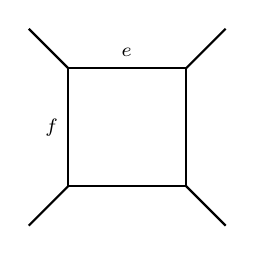
\begin{tikzpicture}
		\draw[thick] (0, 0) -- (1.5, 0) -- (1.5, 1.5) -- (0, 1.5) -- (0, 0);
		\draw[thick] (0, 0) -- (-0.5, -0.5);
		\draw[thick] (1.5, 0) -- (2, -0.5);
		\draw[thick] (1.5, 1.5) -- (2, 2);
		\draw[thick] (0, 1.5) -- (-0.5, 2);
		\draw (-0.2, 0.75) node {$ _f $} (0.75, 1.7) node {$ _e $};
		\end{tikzpicture}
		\caption{$ \mathbb{F}_0 $}
	\end{subfigure}
	\begin{subfigure}{0.45\textwidth}
		\centering
		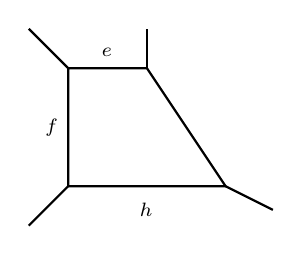
\begin{tikzpicture}
		\draw[thick] (0, 0) -- (0, 1.5) -- (1, 1.5) -- (2, 0) -- (0, 0);
		\draw[thick] (0, 0) -- (-0.5, -0.5);
		\draw[thick] (0, 1.5) -- (-0.5, 2);
		\draw[thick] (1, 1.5) -- (1, 2);
		\draw[thick] (2, 0) -- (2.6, -0.3);
		\draw (-0.2, 0.75) node {$ _f $} (0.5, 1.7) node {$ _e $} (1, -.3) node {$ _h $};
		\end{tikzpicture}
		\caption{$ \mathbb{F}_1 $}
	\end{subfigure}
	\caption{Geometric constructions of (a) $ SU(2)_0 $ and (b) $ SU(2)_\pi $. The fiber $\mathbb{P}^1$ in a Hirzebruch surface $\mathbb{F}_n$ is denoted by $f$, the base $\mathbb{P}^1$ is denoted by $e$, and $h=e+f$ for $\mathbb{F}_1$. } \label{fig:SU2}
\end{figure}
The primitive 2-cycles (or Mori cone generators) in a Hirzebruch surface are the fiber $f$ and the base $e$. The volumes of these 2-cycles are given by
\begin{align}
\left\{
\begin{array}{ll}
\mathbb{F}_0 &: \quad \vol(f) = 2\phi, \quad \vol(e) = 2\phi + m\,, \\
\mathbb{F}_1 &: \quad \vol(f) = 2\phi, \quad \vol(e) = \phi + m\,.
\end{array} \right. 
\end{align}
Here $m$ is a K\"ahler parameter for a non-compact 4-cycle that is identified with the gauge coupling in the gauge theory. This implies that the curve $e$ in each geometry carries charge $+1$ for the $U(1)$ topological symmetry. 

Let us consider a canonically quantized magnetic flux $n\in\mathbb{Z}$ for the $SU(2)$ gauge symmetry in both $\mathbb{F}_0$ and $\mathbb{F}_1$ theories. This magnetic flux can suitably couple to the state coming from a wrapped M2-brane on the fiber curve $f$. This state is a W-boson with gauge charge $+2$ and it feels an integer magnetic flux $2n$, which is compatible with the quantization condition in \eqref{eq:quantization}.

Two theories have different quantization conditions on the background flux $B_m$ for the $U(1)$ topological symmetry. Consider first the theory of $\mathbb{F}_0$. The $e$ curve in this geometry gives rise to a vector multiplet with charge $+2$ for the gauge symmetry and charge $+1$ for the topological symmetry. From the quantization condition \eqref{eq:quantization} with $n\in\mathbb{Z}$, the background flux should be quantized as $B_m\in\mathbb{Z}$. On the other hand, the state associated to the $e$ curve in the theory of $\mathbb{F}_1$ is a hypermultiplet with gauge charge $+1$ and topological charge $+1$. Then the quantization condition \eqref{eq:quantization} requires the background flux to be half-integrally quantized, $B_m\in\mathbb{Z}+1/2$. Hence we find the following quantizations for the magnetic fluxes:
\begin{align}\label{eq:su2_e_shift}
\left\{
\begin{array}{ll}
\mathbb{F}_0 &: \quad n\in\mathbb{Z} \ , \quad B_m \in \mathbb{Z} \\
\mathbb{F}_1 &: \quad n\in\mathbb{Z} \ , \quad B_m \in \mathbb{Z}+1/2\,.
\end{array}\right.
\end{align}

We note however that not all integer/half-integer fluxes $B_m$ are allowed in the blowup equations; the blowup equations only with the consistent magnetic fluxes can be solved to produce the correct BPS spectrum, as discussed in the previous subsection. If one uses other sets of magnetic fluxes, then the solution to the blowup equation will contain some BPS states with negative volumes ${\rm vol}(C)<0$ on the Coulomb branch, which is surely inconsistent. So we first need to identify the consistent magnetic fluxes $B_m$.

Let us try to solve the blowup equation with magnetic fluxes $n\in\mathbb{Z}$ and some $B_m$. The magnetic fluxes result in the shifts of parameters in the North and the South poles as $\phi \to \phi + n \,\epsilon_{1,2}$, $m \to m + B_m\,\epsilon_{1,2}$. The GV-invariant (or the Witten index) can be decomposed into two parts, the perturbative and the instanton parts, as
\begin{align}
	Z_{GV}(\phi,m;\epsilon_1,\epsilon_2) &= \mathcal{Z}_{\rm pert}(\phi;\epsilon_1,\epsilon_2)\cdot \mathcal{Z}_{\rm inst}(\phi,m;\epsilon_1,\epsilon_2) \ , \nonumber \\
	\mathcal{Z}_{\rm pert}(\phi;\epsilon_1,\epsilon_2) & ={\rm PE}\left[-\frac{1+p_1p_2}{(1-p_1)(1-p_2)}e^{-2\phi}\right] \ , \nonumber \\
	\mathcal{Z}_{\rm inst}(\phi,m;\epsilon_1,\epsilon_2) &= \sum_{k=0}^\infty q^k Z_k(\phi; \epsilon_1, \epsilon_2) \ ,
\end{align}
with the instanton fugacity $q\equiv e^{-m}$ and $Z_0=1$. The perturbative part comes from the W-boson (or the M2-brane state on $f$) on the Coulomb branch. Plugging the GV-invariant into \eqref{eq:bleq-GV}, one finds a unity blowup equation that can be expanded in terms of the instanton fugacity as
\begin{align}
\sum_{k,k'=0}^\infty q^{k+k'}\Lambda_{k'} \hat{Z}_k(\phi; \epsilon_1, \epsilon_2)=& \
\sum_{n \in \mathbb{Z}}  \sum_{k_1, k_2=0}^\infty (-1)^n e^{-V}\frac{\hat{\mathcal{Z}}_{\text{pert}}^{(N)}\hat{\mathcal{Z}}_{\text{pert}}^{(S)}}{\hat{\mathcal{Z}}_{\text{pert}}} (q \,p_1^{B_m})^{k_1} (q\, p_2^{B_m})^{k_2}  \\
&\  \times \hat{Z}_{k_1}^{(N)}(\phi + n\epsilon_1 ; \epsilon_1, \epsilon_2 - \epsilon_1) \cdot \hat{Z}^{(S)}_{k_2}(\phi + n\epsilon_2; \epsilon_1 - \epsilon_2, \epsilon_2)\,, \nonumber
\end{align}
with $V$ defined in \eqref{eq:GV-V}, where $\Lambda_0=1$ which is fixed by the zeroth order equation in the expansion. Here, the hatted functions are defined with the shift in the parameter $\epsilon_1$ as
\begin{equation} 
	\hat{f}(\phi,m;\epsilon_1,\epsilon_2)\equiv f(\phi,m;\epsilon_1+2\pi i,\epsilon_2) \ .
\end{equation}

One can extract the $k$-th order of the instanton expansion of this equation, which can be schematically written as
\begin{align}
\Lambda_k(\epsilon_1,\epsilon_2) + \hat{Z}_k(\phi; \epsilon_1, \epsilon_2)
=& ~p_1^{kB_m}\, \hat{Z}_k(\phi; \epsilon_1, \epsilon_2 - \epsilon_1) + p_2^{kB_m}\, \hat{Z}_k(\phi; \epsilon_1 - \epsilon_2, \epsilon_2) \cr
&+ (\text{terms with } \hat{Z}_{r<k} \ \text{and } \Lambda_{r<k})\ .
\end{align}
Here the $k$-instanton partition function $\hat{Z}_k$ at the $k$-th order in the expansion is independent of the background magnetic flux $B_m$ and appears only with a trivial gauge flux $n=0$.
All $\phi$ independent terms in the second line (first by expanding it in $e^{-\phi}$) will be absorbed into $\Lambda_k$. This equation can be solved once we know the solutions $Z_{r}$ at the lower orders $r<k$. In particular, since $\hat{Z}_k$ is independent of $B_m$, when there exist 3 (or more) distinct consistent fluxes $B_m$, we can exactly solve three linearly independent equations for 3 unknown functions, $\hat{Z}_k,\hat{Z}_k^{(N)},$ and $\hat{Z}^{(S)}_k$, and hence find a closed expression for the $k$-instanton partition function $\hat{Z}_k$ at each $k$.

The first order of the blowup equation can be written explicitly as
\begin{align}\label{eq:1-inst-su2}
	\Lambda_1+\hat{Z}_1 =& \  p_1^{B_m}\hat{Z}_1^{(N)}+p_2^{B_m}\hat{Z}_1^{(S)} - \frac{(p_1p_2)^{B_m+1}e^{-2(2+B_m)\phi_1}}{(1-e^{-2\phi})(1-p_1e^{-2\phi})(1-p_2e^{-2\phi})(1-p_1p_2e^{-2\phi})} \nonumber \\
	&- \frac{(p_1p_2)^{B_m-1}e^{-2(2-B_m)\phi_1}}{(1-e^{-2\phi_1})(1-p_1^{-1}e^{-2\phi_1})(1-p_2^{-1}e^{-2\phi_1})(1-(p_1p_2)^{-1}e^{-2\phi_1})} \ .
\end{align}
The last two terms on the right-hand side come from the perturbative parts with the gauge fluxes $n=1$ and $n=-1$ respectively. One can then easily see that if $B_m>2$ or $B_m<-2$, then the last two terms will start with a negative power of $e^{-\phi}$ in the expansion. This means that the solution $\hat{Z}_1$ to the above equation will involve a BPS state of mass $|M|=m+ a \phi$ with a negative coefficient $a$. This is problematic because this state violates the unitarity condition on its mass, i.e. $a\phi\ge0$, on the Coulomb branch parametrized by $\phi>0$ in the UV limit where $m\rightarrow0$. In addition, one can check that this state is not a hypermultiplet and thus there is no associated flop transition. Thus the solution is inconsistent due to the states with  negative masses (or volumes) in the UV limit. This tells us that solving the blowup equations with flux $|B_m|>2$ cannot give the correct BPS partition function for the pure $SU(2)_\theta$ gauge theory.

On the other hand, if $-2\le B_m\le 2$, then the solution will not contain any states with ${\sf{e}}\cdot\phi<0$. Therefore we conclude that the consistent magnetic fluxes for the $SU(2)_0$ and $SU(2)_\pi$ theories are
\begin{align}
\left\{
\begin{array}{ll}
\mathbb{F}_0:~~SU(2)_0 & \quad n\in\mathbb{Z} \ , \ \ B_m = -2,\ -1,\ 0,\ 1, 2 \\
\mathbb{F}_1:~~SU(2)_\pi & \quad n\in\mathbb{Z} \ , \ \  B_m =-\frac{3}{2},\ -\frac{1}{2},\ \frac{1}{2},\ \frac{3}{2}\ .
\end{array}\right. \label{eq:su2 three choices of B}
\end{align}

Since we have more than three sets of consistent fluxes $(n,B_m)$ for both cases, we can compute  a closed expression of the partition function at each instanton order. For example, the 1-instanton partition functions are given as follows:
\begin{align}
Z_1^{SU(2)_0}(\phi; \epsilon_1, \epsilon_2)
&= \frac{p_1 p_2 (1+p_1 p_2)e^{-2\phi}}{(1-p_1)(1-p_2)(1-p_1 p_2 e^{-2\phi})(e^{-2\phi}-p_1p_2)}\ , \label{eq:SU2_0Z-1instanton}\\
Z_1^{SU(2)_\pi}(\phi; \epsilon_1, \epsilon_2)
&= -\frac{p_1^{3/2} p_2^{3/2}(1+e^{-2\phi})e^{-\phi}}{ (1-p_1)(1-p_2) (1-p_1 p_2 e^{-2\phi})(e^{-2\phi}-p_1 p_2)}\ . \label{eq:SU2_piZ-1instanton}
\end{align}
By repeating this procedure for the blowup equations to higher orders in $q$, it is straightforward to obtain the $k$-instanton partition functions $Z_k$. 

We note that though there are many theories which possess three different sets of consistent magnetic fluxes, many of which are discussed in \cite{Kim:2019uqw}, a much larger class of theories do not allow such three distinct sets. However, as discussed in the previous subsection and also in \cite{Huang:2017mis,Gu:2019pqj}, a single unity blowup equation with the consistent magnetic fluxes $(\vec{n},\vec{B})$ is enough to compute the BPS partition function. We will now illustrate this by computing the BPS spectra of the pure $SU(2)_\theta$ theories, using only a single background flux $B_m$ giving a unity blowup equation.

\paragraph{Solving a unity blowup equation}

Let us start with the following ansatz for the GV-invariant.
\begin{align}
	Z_{GV}(\phi,m;\epsilon_{1,2})&={\rm PE}\left[\sum_{j_l,j_r}\sum_{d_1,d_2=0}^\infty(-1)^{2(j_l+j_r)}N_{j_l,j_r}^{(d_1,d_2)} A_{j_l,j_r}(\epsilon_1,\epsilon_2) e^{-d_1{\rm vol}(e)-d_2{\rm vol}(f)}\right] \nonumber \\
	A_{j_l,j_r}(\epsilon_1,\epsilon_2) &\equiv\frac{\chi_{j_l}^{SU(2)}(p_1/p_2)\chi_{j_r}^{SU(2)}(p_1p_2)}{(p_1^{1/2}-p_1^{-1/2})(p_2^{1/2}-p_2^{-1/2})} \ .
\end{align}
Here ${\bf d}=(d_1,d_2)$ denotes the degrees $d_1$ and $d_2$ of 2-cycles $e$ and $f$ respectively. The BPS states with $d_1=0$ at 0-instanton sector are all captured by the perturbative spectrum of the $SU(2)$ theory. The perturbative spectrum then fixes $N_{0,\frac12}^{(0,1)}=1$ and $N_{j_l,j_r}^{(0,d_2)}=0$ for $d_2>1$.

We shall now put the ansatz to the blowup equation and solve it order by order in $d_1$ expansion. Let us first consider the $SU(2)_0$ theory with the background flux $B_m=0$. The equation at $d_1=1$ order is given in \eqref{eq:1-inst-su2}. To solve this equation, we further expand the equation in $d_2$ as
\begin{align}
	\Lambda_1 = &~\hat{Z}^{(N)}_1 + \hat{Z}^{(S)}_1 -\hat{Z}_1 -\big(p_1p_2+(p_1p_2)^{-1}\big)e^{-4\phi}\cr
	&-\frac{(1+p_1)(1+p_2)(1+p_1^3p_2^3)}{p_1^2p_2^2}e^{-6\phi}+\mathcal{O}(e^{-8\phi}) \ .
\end{align}
This equation can be easily solved order by order in $d_2$ or in the powers of $e^{-\phi}$. 

It turns out that this equation uniquely determines all the degeneracies $N_{j_l,j_r}^{(1,d_2)}$, except for the degeneracies $N_{0,\frac12}^{(1,d_2)}$ for all $d_2\ge0$. The result is listed in Table~\ref{table:SU2_0_1inst}. 
\begin{table}[H]
	\centering
	\begin{tabular}{|c|C{25ex}||c|C{25ex}|} \hline
		$\mathbf{d}$ & $\oplus N_{j_l, j_r}^{\mathbf{d}} (j_l, j_r)$ & $\mathbf{d}$ & $\oplus N_{j_l, j_r}^{\mathbf{d}} (j_l, j_r)$ \\ \hline
	 	$ (1, 0) $ & $ N_{0, \frac{1}{2}}^{(1, 0)}(0, \frac{1}{2}) $ & $ (1, 1) $ & $ N_{0, \frac{1}{2}}^{(1, 1)}(0, \frac{1}{2}) \oplus (0, \frac{3}{2}) $ \\ \hline
		$ (1, 2) $ & $ N_{0, \frac{1}{2}}^{(1, 2)}(0, \frac{1}{2}) \oplus (0, \frac{5}{2}) $ & $ (1, 3) $ & $ N_{0, \frac{1}{2}}^{(1, 3)}(0, \frac{1}{2}) \oplus (0, \frac{7}{2}) $ \\ \hline
	\end{tabular}
	\caption{The result of solving the $ SU(2)_0 $ blowup equation at $d_1=1$ order for the background flux $ B_m = 0 $.} \label{table:SU2_0_1inst}
\end{table}
The degeneracies $N_{0,\frac12}^{(1,d_2)}$ are not determined in the 1st order computation because they vanish in the combination $\hat{Z}^{(N)}_1 + \hat{Z}^{(S)}_1 -\hat{Z}_1$ and thus do not appear in the above equation. These undetermined degeneracies at $d_1=1$ order are all fixed by solving the blowup equation in the next order or higher orders: $N_{0,\frac12}^{(1,0)}=1$ and $N_{0,\frac12}^{(1,d_2)}=0$ for $d_2>0$.

We can solve the blowup equation iteratively and compute the degeneracies of higher degree curves.  
The resulting BPS spectra for $ d_1 \leq 2 $, $ d_2 \leq 3 $ are summarized in  Table~\ref{table:SU2_0}. One can readily see that this result agrees with the above result obtained by solving three blowup equations in \eqref{eq:SU2_0Z-1instanton}.
\begin{table}[H]
	\centering
	\begin{tabular}{|c|C{25ex}||c|C{25ex}|} \hline
		$\mathbf{d}$ & $\oplus N_{j_l, j_r}^{\mathbf{d}} (j_l, j_r)$ & $\mathbf{d}$ & $\oplus N_{j_l, j_r}^{\mathbf{d}} (j_l, j_r)$ \\ \hline
		$ (1, 0) $ & $ (0, \frac{1}{2}) $ & $ (1, 1) $ & $ (0, \frac{3}{2}) $ \\ \hline
		$ (1, 2) $ & $ (0, \frac{5}{2}) $ & $ (1, 3) $ & $ (0, \frac{7}{2}) $ \\ \hline
		$ (2, 1) $ & $ (0, \frac{5}{2}) $ & $ (2, 2) $ & $ (0, \frac{5}{2}) \oplus (0, \frac{7}{2}) \oplus (\frac{1}{2}, 4) $ \\ \hline
		$ (2, 3) $ & \multicolumn{3}{c|}{$ (0, \frac{5}{2}) \oplus (0, \frac{7}{2}) \oplus 2(0, \frac{9}{2}) \oplus (\frac{1}{2}, 4) \oplus (\frac{1}{2}, 5) \oplus (1, \frac{11}{2}) $} \\ \hline
	\end{tabular}
	\caption{BPS spectrum of the $ SU(2)_0 $ theory for $ d_1 \leq 2 $, $ d_2 \leq 3 $, where $ \mathbf{d} = (d_1, d_2) $ labels the states from an M2-brane wrapping $ d_1 e + d_2 f $ curve in $ \mathbb{F}_0 $.} \label{table:SU2_0}
\end{table}
\noindent 
Next, consider the $ SU(2)_\pi $ theory with a background magnetic flux $B_m = \frac{1}{2}$. The computation is basically the same as the previous case with $\theta=0$. The blowup equation at $d_1=1$ order is expanded as
\begin{align}
	\Lambda_1 = &~ p_1^{1/2}\hat{Z}^{(N)}_1 + p_2^{1/2}\hat{Z}^{(S)}_1 -\hat{Z}_1 -(p_1p_2)^{1/2}e^{-3\phi}\cr
	&-\frac{1+(1+p_1)(1+p_2)p_1^2p_2^2}{(p_1p_2)^{3/2}}e^{-5\phi}+\mathcal{O}(e^{-7\phi}) \ .
\end{align}
All the degeneracies $N_{j_l,j_r}^{(1,d_2)}$ are uniquely determined by solving this equation, except for the degeneracies $N_{0,0}^{(1,d_2)}$ for all $d_2\ge0$. The undetermined degeneracies $N_{0,0}^{(1,d_2)}$ are also fixed uniquely by solving the equations in higher orders. We list the result for $d_1\le2,d_2\le3$ in Table~\ref{table:SU2_pi}. Like the $SU(2)_0$ case, this result agrees with the expansion of \eqref{eq:SU2_piZ-1instanton}.

\begin{table}[H]
	\centering
	\begin{tabular}{|c|C{25ex}||c|C{25ex}|} \hline
		$\mathbf{d}$ & $\oplus N_{j_l, j_r}^{\mathbf{d}} (j_l, j_r)$ & $\mathbf{d}$ & $\oplus N_{j_l, j_r}^{\mathbf{d}} (j_l, j_r)$ \\ \hline
		$ (1, 0) $ & $ (0, 0) $ & $ (1, 1) $ & $ (0, 1) $ \\ \hline
		$ (1, 2) $ & $ (0, 2) $ & $ (1, 3) $ & $ (0, 3) $ \\ \hline
		$ (2, 2) $ & $ (0, \frac{5}{2}) $ & $ (2, 3) $ & $ (0, \frac{5}{2}) \oplus (0, \frac{7}{2}) \oplus (\frac{1}{2}, 4) $ \\ \hline
	\end{tabular}
	\caption{ BPS spectrum of the $ SU(2)_\pi $  theory for $ d_1 \leq 2 $, $ d_2 \leq 3 $, where $ \mathbf{d} = (d_1, d_2) $ labels the states from an M2-brane wrapping $ d_1 e + d_2 f $ curve in $ \mathbb{F}_1 $.} \label{table:SU2_pi}
\end{table}

\paragraph{Solving a vanishing blowup equation}
In the $ SU(2) $ gauge theories, it is possible to turn on non-canonically quantized magnetic flux as $ n \in \mathbb{Z}+1/2 $ because the W-boson carries charge +2 for the gauge symmetry. Then we can choose $ B_m \in \mathbb{Z} $ which is a consistent quantization for the instanton state corresponding to the curves $ e $  in both $ \mathbb{F}_0 $ and $ \mathbb{F}_1 $. So the magnetic fluxes
\begin{align}\label{eq:su2_vanishing_flux}
n \in \mathbb{Z} + 1/2 \ , \quad
B_m = 0 \ ,
\end{align}
satisfy the quantization conditions for both $ \theta = 0 $ and $ \pi $. These fluxes with the effective prepotential for the $SU(2)$ theories lead to a vanishing blowup equation. We will now show that this vanishing blowup equation alone can be solved with additional geometric data. In fact, we find two independent solutions to the blowup equation and they correspond to respectively the BPS spectrum of the $SU(2)_0$ theory and that of the $SU(2)_\pi$ theory.

Solving the vanishing blowup equation is much harder than solving unity equations because of huge cancellations in the expansion and also non-uniqueness of solutions. Let us start with an ansatz for the GV-invariant as
\begin{align}
Z_{\mathrm{GV}} = \PE\qty[ \,\sum_{j_l, j_r} \sum_{d_1, d_2 = 0}^\infty (-1)^{2(j_l + j_r)} N_{j_l, j_r}^{(d_1, d_2)} A_{j_l, j_r}(\epsilon_1, \epsilon_2) e^{-(d_1 m + d_2 \phi)} ] \, .
\end{align}
As discussed in \cite{Gu:2017ccq}, the spins of a degree $(d_1,d_2)$ state are bounded as
\begin{align}
j_l &\leq \frac{C^2\! +\! K_S \cdot C}{2} \!+\! 1 = \frac{d_1 d_2 \!-\! 2d_1^2 \!-\! d_2\!+\!2}{2} \, , \cr
 j_r &\leq \frac{C^2 \!-\! K_S \cdot C}{2} = \frac{d_1 d_2 \!-\! 2d_1^2 \!+\! d_2}{2}\, ,
\end{align}
where $ C $ is a curve with volume $ d_1 m + d_2 \phi $ and $ K_S $ is the canonical class in $ \mathbb{F}_0 $ or $ \mathbb{F}_1 $.

The zeroth-order in the expansion of the blowup equation is
\begin{align}
\sum_{n \in \{ \pm 1/2 \}} (-1)^n e^{-V} \frac{\hat{\mathcal{Z}}_{\mathrm{pert}}^{(N)} \hat{\mathcal{Z}}_{\mathrm{pert}}^{(S)}}{\hat{\mathcal{Z}}_{\mathrm{pert}}} = 0 \, ,
\end{align}
which is automatically satisfied by the perturbative spectrum $ N_{0, 1/2}^{(0, 2)} = 1 $. The 1st order blowup equation with $d_1=1$ is then given by
\begin{align}
\sum_{n \in \{ \pm 1/2 \}} (-1)^n e^{-V} \frac{\hat{\mathcal{Z}}_{\mathrm{pert}}^{(N)} \hat{\mathcal{Z}}_{\mathrm{pert}}^{(S)}}{\hat{\mathcal{Z}}_{\mathrm{pert}}} \qty(\hat{Z}_1^{(N)} + \hat{Z}_1^{(S)}) = 0 \, .
\end{align}
This equation for each $ d_2 $ can be rephrased in terms of the multiplicities $ N_{j_l,j_r}^{(1, d_2)} $ as
\begin{align}\label{eq:su2_vanishing_1st}
& \sum_{j_l, j_r} (-1)^{2(j_l + j_r)} N_{j_l, j_r}^{(1, d_2)} \qty( A_{j_l, j_r}(\epsilon_1, \epsilon_2/\epsilon_1) p_1^{-d_2/2} + A_{j_l, j_r}(\epsilon_1/\epsilon_2, \epsilon_2) p_2^{-d_2/2} -  A_{j_l, j_r}(\epsilon_1, \epsilon_2)) \nonumber \\
& = \sum_{j_l, j_r} (-1)^{2(j_l + j_r)} N_{j_l, j_r}^{(1, d_2)} \qty( A_{j_l, j_r}(\epsilon_1, \epsilon_2/\epsilon_1) p_1^{d_2/2} + A_{j_l, j_r}(\epsilon_1/\epsilon_2, \epsilon_2) p_2^{d_2/2} -  A_{j_l, j_r}(\epsilon_1, \epsilon_2)) \, .
\end{align}
It turns out that this equation is not enough to fix the multiplicities $ N_{j_l, j_r}^{(1, d_2)} $, and in fact it has infinitely many solutions. For example, if $ N_{j_l,j_r}^{(1, d_2)}=c^{(d_2)} $ with an integer number $c^{(d_2)}$ is a solution, then $ N_{j_l,j_r}^{(1, d_2)} =2c^{(d_2)}$ is also another solution. 
We thus need to solve higher order equations to determine them.

The 2nd order of the blowup equation can be written as
\begin{align}
\sum_{n \in \{ \pm 1/2 \}} (-1)^n e^{-V} \frac{\hat{\mathcal{Z}}_{\mathrm{pert}}^{(N)} \hat{\mathcal{Z}}_{\mathrm{pert}}^{(S)}}{\hat{\mathcal{Z}}_{\mathrm{pert}}} & \qty( \hat{Z}_2^{(N)} +  \hat{Z}_2^{(S)} +  \hat{Z}_1^{(N)} \hat{Z}_1^{(S)} ) \nonumber \\
& + \sum_{n \in \{\pm 3/2\}} (-1)^n e^{-V} \frac{\hat{\mathcal{Z}}_{\mathrm{pert}}^{(N)} \hat{\mathcal{Z}}_{\mathrm{pert}}^{(S)}}{\hat{\mathcal{Z}}_{\mathrm{pert}}}
= 0 \ .
\end{align}
Unfortunately, this equation does not help us to fix the degeneracies $ N_{j_l, j_r}^{(1, d_2)} $ because they do not appear in this order. We need the blowup equation at higher orders to fully fix $ N_{j_l, j_r}^{(1, d_2)}$. We find that at the order of the blowup equation involving $ N_{j_l, j_r}^{(4, 10)} $, the degeneracy $ N_{j_l, j_r}^{(1, 1)} $ is first fixed to be
\begin{align}
N_{j_l, j_r}^{(1, 1)} =0\ ,\quad\text{except for} ~~
N_{0, 0}^{(1, 1)} = \Bigg\{
\begin{array}{ll}
1 & \quad \text{when~} \theta=\pi \\
0 & \quad \text{when~}\theta=0
\end{array} \ .
\end{align}
Here we fixed the discrete theta angles from the geometric information: $ N_{j_l, j_r}^{(1, 1)} = 0 $ for the $ SU(2)_0 $ theory, while $ N_{0, 0}^{(1, 1)} =1 $ for the $ SU(2)_\pi $ theory. 

Now consider the $ SU(2)_0 $ theory. Solving the blowup equation at the order having terms of $ N_{j_l, j_r}^{(4, 12)} $ again gives two sets of solutions: one with $ N_{j_l, j_r}^{(1, 2)} = 0 $ for all $ (j_l, j_r) $ and the other with $ N_{j_l, j_r}^{(1, 2)} = 0 $ but $ N_{0, \frac{1}{2}}^{(1, 2)} = 1 $. However, the geometric realization suggests that there exists a BPS state with charge $ m + 2\phi $, so only the second solution is acceptable. The next order blowup equation which contains $ N_{j_l, j_r}^{(4, 13)} $ gives $ N_{j_l, j_r}^{(1, 3)} = 0 $ for all $ (j_l, j_r) $. Now to fix $ N_{j_l, j_r}^{(1, 4)} $, instead of calculating higher order equations, one can use other consistency conditions. First, we know from geometry that there are effective curves with volume $ m + 4\phi $. In addition, the blowup equation yields that $ N_{j_l, j_r}^{(1, 4)} = 0 $ for $ (j_l, j_r) \neq (0, \frac{3}{2}) $ and  $N_{1,\frac{15}{2}}^{(3,12)} = 1 - N_{0,\frac{3}{2}}^{(1, 4)} $. Notably, $ N_{1,\frac{15}{2}}^{(3,12)} $ must be a non-negative integer and $ N_{0,\frac{3}{2}}^{(1, 4)} \neq 0 $ from geometry. Therefore the only possible solution is $ N_{0,\frac{3}{2}}^{(1, 4)} = 1 $. This result reproduces all the BPS states of the $SU(2)_0$ theory up to $(d_1,d_2)=(1,4)$. In this way, a vanishing blowup equation together with other consistency conditions can determine the BPS spectrum in this theory. We expect other higher degree states can also be captured by solving higher order blowup equations in this manner. 

Next, consider the $ SU(2)_\pi $ theory. The blowup equation at the order containing $ N_{j_l, j_r}^{(4, 11)} $ fixes $ N_{j_l, j_r}^{(1, 2)} = 0 $ for all $ (j_l, j_r) $. The higher order equations containing $ N_{j_l, j_r}^{(4, 14)} $ has two sets of solutions: one with $ N_{j_l, j_r}^{(1, 3)} = 0 $ for all $ (j_l, j_r) $, and the other one with $ N_{j_l, j_r}^{(1, 3)} = 0 $ but $ N_{0, 1}^{(1, 3)} = 1 $. Also, the geometry of $\mathbb{F}_1$ says that there is a state with charge $ m + 3\phi $, so only the second one is acceptable. The next order equation containing $ N_{j_l, j_r}^{(4, 15)} $ fixes $ N_{j_l, j_r}^{(1, 4)} = 0 $. It is also possible to fix $ N_{j_l, j_r}^{(1, 4)} $ by consistency conditions instead of calculating higher order equations. The blowup equation fixes $ N_{j_l, j_r}^{(1, 4)} = 0 $  for $ (j_l, j_r) \neq (0, \frac{3}{2}) $, and $N_{1,\frac{15}{2}}^{(3,12)} = - N_{0,\frac{3}{2}}^{(1, 4)}$, from which the only possible solution is $ N_{0,\frac{3}{2}}^{(1, 4)} = 0 $. This result agrees with the spectrum of the $ SU(2)_\pi $ theory that we computed above using unity bloup equations. 

These computations show that, although the BPS spectrum is not completely determined only by solving vanishing blowup equations, we may be able to uniquely determine the BPS degeneracies by requiring the solution of the vanishing blowup equations to be physically or geometrically consistent.


\subsubsection{\texorpdfstring{5d pure $SU(3)_{\kappa \leq 7}$}{5d pure SU(3)k}}\label{sec:su3_k}

Let us now discuss rank-2 theories. A non-trivial example is the pure $SU(3)$ gauge theory at the Chern-Simons level $ \kappa $. When $ \kappa $ is even, it is geometrically engineered as
\begin{align}\label{eq:su3_even_geo}
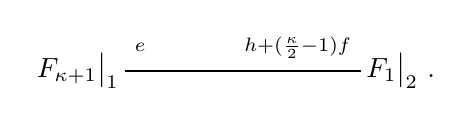
\begin{tikzpicture}
\draw[thick](-3,0)--(0,0);	
\node at(-3.6,0) {$\mathbb{F}_{\kappa+1}{}\big|_1$};
\node at(-2.8,0.3) {${}_e$};
\node at(0.5,0) {$\mathbb{F}_{1}{}\big|_2$\ .};
\node at(-0.8,0.3) {${}_{h+(\frac{\kappa}{2}-1)f}$};
\end{tikzpicture}
\end{align}
Whereas, if $\kappa$ is odd, it is engineered by
\begin{align}\label{eq:su3_odd_geo}
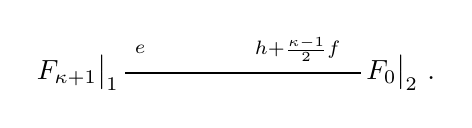
\begin{tikzpicture}
\draw[thick](-3,0)--(0,0);	
\node at(-3.6,0) {$\mathbb{F}_{\kappa+1}{}\big|_1$};
\node at(-2.8,0.3) {${}_e$};
\node at(0.5,0) {$\mathbb{F}_{0}{}\big|_2$\ .};
\node at(-0.8,0.3) {${}_{h+\frac{\kappa-1}{2}f}$};
\end{tikzpicture}
\end{align}
Each geometry contains three primitive curves: the fiber $f_1$ in $\mathbb{F}_{n_1}|_1$, the fiber $f_2$ and the base $e_2$ in $\mathbb{F}_{n_2}|_2$.
The volumes of the primitive 2-cycles are
\begin{align}
&\vol(f_1) = 2\phi_1 - \phi_2, \quad
\vol(f_2) = -\phi_1 + 2\phi_2, \nonumber\\
&\vol(e_2) = \left\{ \begin{array}{ll} \left(1-\tfrac{\kappa}{2}\right)\phi_1+\phi_2 + m& \ \ {\rm for \ even}\ \kappa \\
	\frac{1-\kappa}{2}\phi_1+2\phi_2 + m & \ \ {\rm for \ odd}\ \kappa 
	\end{array}\right. \ .
\end{align}
These theories with CS level $|\kappa|\le9$ have UV completions \cite{Jefferson:2018irk,Bhardwaj:2019jtr}. The 5-brane webs for $|\kappa|\le 7$ and $|\kappa|=9$ have been constructed in \cite{Hayashi:2018lyv}. 

Surprisingly the BPS spectra of the  $SU(3)_\kappa$ theories for all $|\kappa|\le 9$ can be computed by employing our bootstrapping approach explained above. The $SU(3)_8$ theory is of particular interest. Unlike other $\kappa$, this theory at $\kappa=8$ has no consistent geometric realization \cite{Jefferson:2018irk,Bhardwaj:2019jtr,Bhardwaj:2020gyu} and also its 5-brane web is unknown yet. Moreover the usual ADHM construction for instantons in this theory does not work. So it was a quite challenging task to compute its BPS partition function. The $SU(3)_8$ theory and its blowup equations will be discussed separately in subsection~\ref{sec:SU3_8}. The $SU(3)_9$ theory, which is a KK theory, will be discussed in subsection~\ref{subsubsec:SU3/Z2}.

In this subsection, we will illustrate how to bootstrap the BPS spectra of  $|\kappa| \le 7$ theories and their dual theories using the blowup equations as well as their geometric descriptions.

Consider the $SU(3)_\kappa$ theory put on the blowup $\hat{\mathbb{C}}_2$. We turn on the magnetic flux $\textsf{F}=(n_1,n_2,B_m)$ for two Hirzebruch surfaces and a non-compact divisor of the non-normalizable K\"ahler parameter $m$. The quantization conditions for the fluxes are given by their intersections with the primitive 2-cycles as
\begin{align}
	&\textsf{F}\cdot f_1 = 2n_1-n_2\ \in \ \mathbb{Z} \ , \qquad \textsf{F}\cdot f_2 = 2n_2-n_1 \ \in \ \mathbb{Z} \nonumber \ ,\\
	&  \textsf{F}\cdot e_2 = \left\{ \begin{array}{ll} \left(1-\tfrac{\kappa}{2}\right)n_1+n_2 + B_m \ \in \ \mathbb{Z}+\frac{1}{2} & \ \ {\rm for \ even}\ \kappa \\
	\frac{1-\kappa}{2}n_1+2n_2 + B_m \ \in \ \mathbb{Z} & \ \ {\rm for \ odd}\ \kappa 
	\end{array}\right. \ ,
\end{align}
which follow from the geometric quantization condition \eqref{eq:quantization} together with the self-intersections of the curves, $f_1^2 = f_2 ^2 = 0$ and $e_2^2 = -1$ for even $\kappa$ and $e_2^2=0$ for odd $\kappa$. Each theory has 3 or more sets of magnetic fluxes satisfying the quantization conditions. We can use, for example, the following fluxes for solving the blowup equations:
\begin{equation}\label{eq:su3_r}
	n_1,n_2 \in \mathbb{Z} \quad {\rm and} \quad B_m = \left\{
\begin{array}{ll}
-\frac{1}{2}, \frac{1}{2}, \frac{3}{2} & \quad \kappa = 0, 2, 4, 6 \\
-1, 0, 1 & \quad \kappa = 1, 3, 5, 7\ .
\end{array}\right.
\end{equation}

Let us now consider the Coulomb branch of the theory where $2\phi_1-\phi_2 \ge0$ and $2\phi_2-\phi_1\ge0$ with $\phi_1,\phi_2>0$. The effective prepotential $\mathcal{E}$ on the Coulomb branch takes the following form
\begin{align}\label{eq:SU3_k_prepotential}
\mathcal{E} &= \frac{1}{\epsilon_1 \epsilon_2} 
\left( \mathcal{F} - \frac{\epsilon_1^2  + \epsilon_2^2}{12}(\phi_1 + \phi_2) +\epsilon_+^2 (\phi_1 + \phi_2) \right), \\ 
6\,\mathcal{F} &= 6 m(\phi_1^2 - \phi_1 \phi_2 + \phi_2^2)+ 3\kappa \phi_1 \phi_2(\phi_1 - \phi_2) + 8 \phi_1^3 - 3\phi_1^2 \phi_2 - 3\phi_1 \phi_2^2 + 8\phi_2^3\, ,\nonumber
\end{align}
where $m$ is the gauge coupling. The GV-invariant of this theory can be factorized as
\begin{align}
Z_{GV}(\phi_i, m; \epsilon_1, \epsilon_2) &= \mathcal{Z}_{\mathrm{pert}}(\phi_i; \epsilon_1, \epsilon_2) \cdot \mathcal{Z}_{\mathrm{inst}}(\phi_i, m; \epsilon_1, \epsilon_2) \ , \nonumber  \\
\mathcal{Z}_{\mathrm{pert}}(\phi_i; \epsilon_1, \epsilon_2) &= \PE \qty[-\frac{1+p_1 p_2}{(1-p_1)(1-p_2)} \qty(e^{-(2\phi_1 - \phi_2)} + e^{-(2\phi_2-\phi_1)} + e^{-(\phi_1 + \phi_2)})] \ , \nonumber \\
\mathcal{Z}_{\mathrm{inst}}(\phi_i, m; \epsilon_1, \epsilon_2) &= \sum_{k=0}^{\infty} q^k Z_k(\phi; \epsilon_1, \epsilon_2) \ ,
\label{eq:SU3_k_GV}
\end{align}
with the instanton fugacity $ q = e^{-m} $ and $ Z_0 = 1 $. 

We can then write the blowup equation for the $SU(3)_\kappa$ theory as
\begin{align}
\sum_{k, k'=0}^{\infty} q^{k+k'} \Lambda_{k'} \hat{Z}_k &= \sum_{\vec{n}\in \mathbb{Z}^2}\sum_{k_1,k_2=0}^\infty (-1)^{\abs{\vec{n}}} e^{-V} \frac{\mathcal{Z}_{\mathrm{pert}}^{(N)} \mathcal{Z}_{\mathrm{pert}}^{(S)}}{\mathcal{Z}_{\mathrm{pert}}} (q \,p_1^{B_m})^{k_1} \hat{Z}^{(N)}_{k_1} \cdot (q \,p_2^{B_m})^{k_2} \hat{Z}^{(S)}_{k_2} \ .
\end{align}
Again, the blowup equation at the $ k $-th order can be written as
\begin{align}\label{eq:su3_k_kinst}
\Lambda_k(m; \epsilon_1, \epsilon_2) + \hat{Z}_k(\phi_i, \epsilon_1, \epsilon_2)
=&~ p_1^{kB_m} \hat{Z}_k(\phi_i, \epsilon_1, \epsilon_2 - \epsilon_1) + p_2^{kB_m}\hat{Z}_k(\phi_i, \epsilon_1 - \epsilon_2, \epsilon_2) \nonumber \\
& + (\text{terms with } Z_{r<k} \text{ and } \Lambda_{r<k})\ .
\end{align}
The $ \Lambda_0 $ factor is then fixed to be 1 from the zeroth order expansion. In $ q^1 $ order, the blowup equation is given by
\begin{align}\label{eq:su3_k_1inst}
\Lambda_1 + \hat{Z}_1(\phi_i, \epsilon_1, \epsilon_2)
= ~& p_1^{B_m} \hat{Z}_1(\phi_i, \epsilon_1, \epsilon_2 - \epsilon_1) + p_2^{B_m} \hat{Z}_1(\phi_i, \epsilon_1 - \epsilon_2, \epsilon_2) \nonumber \\
& +  \sum_{\vec{n} \in S_1} q^{-1} e^{-V} \frac{\mathcal{Z}_{\mathrm{pert}}^{(N)} \mathcal{Z}_{\mathrm{pert}}^{(S)}}{\mathcal{Z}_{\mathrm{pert}}} \ ,
\end{align}
where the last term comes from the contribution with $k_1=k_2=0$ and $n_1^2 - n_1 n_2 +n_2^2 =1$ which is solved for $(n_1,n_2)\in S_1 = \{\pm(1, 1), \pm(1, 0), \pm(0, 1) \}$.

The three choices of $ B_m $ given in \eqref{eq:su3_r} provide three linearly independent  algebraic equations for $\hat{Z}_k(\phi_i, \epsilon_1, \epsilon_2)$ at each $k$-th order.
They allow us to find a closed form of $\hat{Z}_k(\phi_i, \epsilon_1, \epsilon_2)$. Thus, the $k$-instanton partition function $Z_k(\phi_i, \epsilon_1, \epsilon_2)$ for the $SU(3)_\kappa$ theory at $|\kappa|\le 7$ can be computed by recursively solving three blowup equations with $B_m$'s in  \eqref{eq:su3_r}. In \cite{Kim:2019uqw}, the partition functions for $|\kappa|\le 3$ were computed in this manner and checked against the results from the ADHM calculations.

The instanton partition function for the $SU(3)_4$ theory can be computed by solving the blowup equations similarly to the $ \abs{\kappa} \leq 3 $ cases. Using the effective prepotential \eqref{eq:SU3_k_prepotential} and consistent magnetic fluxes \eqref{eq:su3_r}, we solve the blowup equations in terms of volumes of primitive 2-cycles
\begin{align}\label{eq:vol of 2-cycles for SU3_4}
\vol(f_1) = 2\phi_1 - \phi_2 \, , \quad
\vol(f_2) = -\phi_1 + 2\phi_2 \, , \quad
\vol(e_2) = -\phi_1 + \phi_2 + m \, .
\end{align}
Instead of giving an explicit form of the partition function, we list some BPS states in Table~\ref{table:SU(3)_4}.\footnote{As the BPS spectrum in Table~\ref{table:SU(3)_4} is expressed as the expansion of 2-cycles, one can reconstruct the partition function given in terms of dynamical variables, by substituting the 2-cycles with \eqref{eq:vol of 2-cycles for SU3_4}. Likewise, one can also rewrite the partition function given in terms of dynamical variables as the BPS spectrum, by first converting them into the 2-cycles and then expanding the 2-cycles.}
\begin{table}
	\centering
	\begin{tabular}{|c|C{28ex}||c|C{28ex}|} \hline
		$ \mathbf{d} $ & $\oplus N_{j_l, j_r}^{\mathbf{d}} (j_l, j_r)$ & $ \mathbf{d} $ & $\oplus N_{j_l, j_r}^{\mathbf{d}} (j_l, j_r)$ \\ \hline
		$ (1, 0, 0) $ & $ (0, 0) $ & $ (1, 0, 1) $ & $ (0, 1) $ \\ \hline
		$ (1, 0, 2) $ & $ (0, 2) $ & $ (1, 0, 3) $ & $ (0, 3) $ \\ \hline
		$ (1, 1, 0) $ & $ (0, 0) $ & $ (1, 1, 1) $ & $ (0, 0) \oplus (0, 1) $ \\ \hline
		$ (1, 1, 2) $ & $ (0, 1) \oplus (0, 2) $ & $ (1, 1, 3) $ & $ (0, 2) \oplus (0, 3) $ \\ \hline
		$ (1, 2, 1) $ & $ (0, 1) $ & $ (1, 2, 2) $ & $ (0, 0) \oplus (0, 1) \oplus (0, 2) $ \\ \hline
		$ (1, 2, 3) $ & $ (0,1) \oplus (0,2) \oplus (0,3) $ & $ (1, 3, 2) $ & $ (0, 1) \oplus (0, 2) $ \\ \hline
		$ (1, 3, 3) $ & $ (0,0) \oplus (0,1) \oplus (0,2) \oplus (0,3) $ & $ (2, 0, 2) $ & $ (0, \frac{5}{2}) $ \\ \hline
		$ (2, 0, 3) $ & $ (0,\frac{5}{2}) \oplus (0,\frac{7}{2}) \oplus (\frac{1}{2},4) $ & $ (2, 1, 2) $ & $ (0, \frac{3}{2}) \oplus (0, \frac{5}{2}) $ \\ \hline
		$ (2, 1, 3) $ & $ (0,\frac{3}{2}) \oplus 3(0,\frac{5}{2}) \oplus 2(0,\frac{7}{2}) \oplus (\frac{1}{2},3) \oplus (\frac{1}{2},4) $ & $ (2, 2, 2) $ & $ (0,\frac{1}{2}) \oplus (0,\frac{3}{2}) \oplus (0,\frac{5}{2}) $ \\ \hline
		$ (2, 2, 3) $ & $ (0,\frac{1}{2}) \oplus 3(0,\frac{3}{2}) \oplus 4(0,\frac{5}{2}) \oplus 2(0,\frac{7}{2}) \oplus (\frac{1}{2},2) \oplus (\frac{1}{2},3) \oplus (\frac{1}{2},4) $ & $ (2, 3, 2) $ & $ (0,\frac{1}{2}) \oplus (0,\frac{3}{2}) \oplus (0,\frac{5}{2}) $ \\ \hline
		$ (2, 3, 3) $ & $ 3(0,\frac{1}{2}) \oplus 4(0,\frac{3}{2}) \oplus 4(0,\frac{5}{2}) \oplus 2(0,\frac{7}{2}) \oplus (\frac{1}{2},1) \oplus (\frac{1}{2},2) \oplus (\frac{1}{2},3) \oplus (\frac{1}{2},4) $ & $ (3, 0, 3) $ & $ (0, 3) \oplus (\frac{1}{2}, \frac{9}{2}) $ \\ \hline
		$ (3, 1, 3) $ & $ (0,2) \oplus 2(0,3) \oplus (0,4) \oplus (\frac{1}{2},\frac{7}{2}) \oplus (\frac{1}{2},\frac{9}{2}) $ & $ (3, 2, 3) $ & $ (0,1) \oplus 2(0,2) \oplus 3(0,3) \oplus (0,4) \oplus (\frac{1}{2},\frac{5}{2}) \oplus (\frac{1}{2},\frac{7}{2}) \oplus (\frac{1}{2},\frac{9}{2}) $ \\ \hline
		$ (3, 3, 3) $ & \multicolumn{3}{C{68.5ex}|}{$ \! (0,0) \oplus 2(0,1) \oplus 3(0,2) \oplus 3(0,3) \oplus (0,4) \oplus (\frac{1}{2},\frac{3}{2}) \oplus (\frac{1}{2},\frac{5}{2}) \oplus (\frac{1}{2},\frac{7}{2}) \oplus (\frac{1}{2},\frac{9}{2}) \! $} \\ \hline
	\end{tabular}
	\caption{BPS spectrum of $SU(3)_4$ for $ d_i \leq 3 $. Here, $\mathbf{d} = (d_1, d_2, d_3)$ labels the BPS states with charge $d_1 e_2 + d_2 f_1 + d_3 f_2$.} \label{table:SU(3)_4}
\end{table}

The $ SU(3)_5 $ theory is dual to the $ Sp(2)_\pi $ gauge theory, so they can provide a non-trivial check for the validity of the blowup equations. In the geometry \eqref{eq:su3_odd_geo} with $\kappa=5$, this duality is realized as the base-fiber duality exchanging two curve classes $e_2$ and $f_2$ in $\mathbb{F}_0$. The map between the parameters in the $ SU(3)_5 $ theory and those in the $ Sp(2)_\pi $ theory can be easily found from the geometric realization. The volumes of 2-cycles in the $ SU(3) $ frame are
\begin{align}\label{eq:su3_5_vol}
\vol(f_1)= 2 \phi_1 - \phi_2, \quad
\vol(f_2) = -\phi_1 + 2\phi_2, \quad
\vol(e_2) = -2\phi_1 + 2\phi_2 + m\ ,
\end{align}
while those in the $ Sp(2) $ frame after exchanging $e_2$ and $f_2$ are
\begin{align}
\vol(f_1) = 2\phi_1 - \phi_2, \quad
\vol(f_2) = -2\phi_1 + 2\phi_2, \quad
\vol(e_2) = -\phi_1 + 2\phi_2 + m\ .
\end{align}
From this, we find a natural map between the parameters in two dual frames as \cite{Gaiotto:2015una, Hayashi:2016abm, Hayashi:2018lyv}
\begin{align}
\phi_1^{SU} &= \phi_1^{Sp} + \frac{1}{3} m^{Sp} \ , \quad \phi_2^{SU} = \phi_2^{Sp} + \frac{2}{3} m^{Sp} \ ,\quad
m^{SU} = -\frac{2}{3} m^{Sp}\ . \label{eq:SU3 and Sp2 duality map}
\end{align}

The effective prepotential of the $Sp(2)_\pi$ theory on the Coulomb branch is written as
\begin{align}
\mathcal{E} &= \frac{1}{\epsilon_1\epsilon_2}\left(\mathcal{F} -\frac{\epsilon_1^2+\epsilon_2^2}{12}(\phi_1+\phi_2) + \epsilon_+^2(\phi_1+\phi_2)\right) \ , \nonumber \\
6\mathcal{F}
 &= 6m (2\phi_1^2 - 2\phi_1 \phi_2 + \phi_2^2)+8\phi_1^3 + 12\phi_1^2 \phi_2 - 18\phi_1 \phi_2^2 + 8\phi_2^3 \ ,
\end{align}
where $ m $ is the $ Sp(2) $ gauge coupling. One can easily check that this $\mathcal{E}$ of the $ Sp(2)_\pi $ theory coincides with that of the $ SU(3)_5 $ theory in \eqref{eq:SU3_k_prepotential} under the above parameter map up to terms independent of the dynamical K\"ahler parameters. The perturbative GV-invariants of the $Sp(2)_\pi$ gauge theory is
\begin{align}
	\mathcal{Z}_{\rm pert} = {\rm PE} \left[ -\frac{1+p_1p_2}{(1-p_1)(1-p_2)}\left(e^{-2\phi_1}+e^{-\phi_2}+e^{-(2\phi_2-2\phi_1)}+e^{-(2\phi_1-\phi_2)}\right)\right] \ .
\end{align} 

In the $ Sp(2) $ frame, there are three (and more) sets of consistent fluxes respecting the $ Sp(2) $ structure:
\begin{align}
n_1,n_2 \in \mathbb{Z} \ , \quad B_m = -1, 0, 1 \, .
\end{align}
The three sets of unity blowup equations from these magnetic fluxes can be easily solved and the solution provides a closed expression of the instanton partition function of the $ Sp(2)_\pi $ theory at each instanton order. We checked that the result perfectly matches the BPS states captured by the $ SU(3)_5 $ calculation under the parameter map \eqref{eq:SU3 and Sp2 duality map} in the K\"ahler parameter expansion. Instead of giving explicit forms of  the instanton partition functions, we list BPS spectrum up to 3-instanton order in Table~\ref{table:SU(3)_5}.
\begin{table}
	\centering
	\begin{tabular}{|c|C{28ex}||c|C{28ex}|} \hline
		$ \mathbf{d} $ & $\oplus N_{j_l, j_r}^{\mathbf{d}} (j_l, j_r)$ & $ \mathbf{d} $ & $\oplus N_{j_l, j_r}^{\mathbf{d}} (j_l, j_r)$ \\ \hline
		$ (1, 0, 0) $ & $ (0, \frac{1}{2}) $ & $ (1, 0, 1) $ & $ (0, \frac{3}{2}) $ \\ \hline
		$ (1, 0, 2) $ & $ (0, \frac{5}{2}) $ & $ (1, 1, 0) $ & $ (0, \frac{1}{2}) $ \\ \hline
		$ (1, 1, 1) $ & $ (0, \frac{1}{2}) \oplus (0, \frac{3}{2}) $ & $ (1, 1, 2) $ & $ (0, \frac{3}{2}) \oplus (0, \frac{5}{2}) $ \\ \hline
		$ (1, 2, 0) $ & $ (0, \frac{1}{2}) $ & $ (1, 2, 1) $ & $ (0, \frac{1}{2}) \oplus (0, \frac{3}{2}) $ \\ \hline
		$ (1, 2, 2) $ & $ (0, \frac{1}{2}) \oplus (0, \frac{3}{2}) \oplus (0, \frac{5}{2}) $ & $ (2, 0, 1) $ & $ (0, \frac{5}{2}) $ \\ \hline
		$ (2, 0, 2) $ & $ (0, \frac{5}{2}) \oplus (0, \frac{7}{2}) \oplus (\frac{1}{2}, 4) $ & $ (2, 1, 1) $ & $ (0, \frac{3}{2}) \oplus (0, \frac{5}{2}) $ \\ \hline
		$ (2, 1, 2) $ & $ (0, \frac{3}{2}) \oplus 3(0, \frac{5}{2}) \oplus 2(0, \frac{7}{2}) \oplus (\frac{1}{2}, 3) \oplus (\frac{1}{2}, 4) $ & $ (2, 2, 1) $ & $ (0, \frac{1}{2}) \oplus (0, \frac{3}{2}) \oplus (0, \frac{5}{2}) $ \\ \hline
		$ (2, 2, 2) $ & $ (0, \frac{1}{2}) \oplus 3(0, \frac{3}{2}) \oplus 4(0, \frac{5}{2}) \oplus 2(0, \frac{7}{2}) \oplus (\frac{1}{2}, 2) \oplus (\frac{1}{2}, 3) \oplus (\frac{1}{2}, 4) $ & $ (3, 0, 1) $ & $ (0, \frac{7}{2}) $ \\ \hline
		$ (3, 0, 2) $ & $ (0,\frac{5}{2}) \oplus (0,\frac{7}{2}) \oplus 2(0,\frac{9}{2}) \oplus (\frac{1}{2},4) \oplus (\frac{1}{2},5) \oplus (1,\frac{11}{2}) $ & $ (3, 1, 1) $ & $ (0,\frac{5}{2}) \oplus (0,\frac{7}{2}) $ \\ \hline
		$ (3, 1, 2) $ & $ (0,\frac{3}{2}) \oplus 3(0,\frac{5}{2}) \oplus 5(0,\frac{7}{2}) \oplus 3(0,\frac{9}{2}) \oplus	(\frac{1}{2},3) \oplus 3(\frac{1}{2},4) \oplus 2(\frac{1}{2},5) \oplus (1,\frac{9}{2}) \oplus (1,\frac{11}{2}) $ & $ (3, 2, 1) $ & $ (0,\frac{3}{2}) \oplus (0,\frac{5}{2}) \oplus (0,\frac{7}{2}) $ \\ \hline
		$ (3, 2, 2) $ & \multicolumn{3}{C{68ex}|}{$ (0,\frac{1}{2}) \oplus 3(0,\frac{3}{2}) \oplus 8(0,\frac{5}{2}) \oplus 7(0,\frac{7}{2}) \oplus 4(0,\frac{9}{2}) \oplus (\frac{1}{2},2) \oplus 3(\frac{1}{2},3) \oplus 4(\frac{1}{2},4) \oplus 2(\frac{1}{2},5) \oplus (1,\frac{7}{2}) \oplus (1,\frac{9}{2}) \oplus (1,\frac{11}{2}) $} \\ \hline
	\end{tabular}
	\caption{BPS spectrum of $SU(3)_5$ for $d_1 \leq 3$ and $ d_2, d_3 \leq 2 $. Here, $\mathbf{d} = (d_1, d_2, d_3)$ labels the BPS states with charge $d_1 e_2 + d_2 f_1 + d_3 f_2$.} \label{table:SU(3)_5}
\end{table}

In the case of $ \kappa = 6 $, one should be careful about the $ \Lambda $ factor. When background magnetic flux is $ B_m = 3/2 $, the last term of \eqref{eq:su3_k_1inst} in the K\"ahler parameter expansion  contains a $ \phi_i $ independent term :
\begin{align}
-p_1^{1/2} p_2^{1/2}\ \in\ \sum_{\vec{n} \in S_1} q^{-1} e^{-V} \frac{\mathcal{Z}_{\mathrm{pert}}^{(N)} \mathcal{Z}_{\mathrm{pert}}^{(S)}}{\mathcal{Z}_{\mathrm{pert}}} \ .
\end{align}
This term should be absorbed into $ \Lambda_1 $ on the left side of \eqref{eq:su3_k_1inst}. Thus we have
\begin{align}
&\Lambda_1 = 0 \quad \text{for} \quad B_m = \pm \tfrac{1}{2} \ , \qquad \Lambda_1 = -p_1^{1/2} p_2^{1/2} \quad \text{for} \quad B_m = \tfrac{3}{2} \ .
\end{align}
Then the solution $ Z_1(\phi_i; \epsilon_1, \epsilon_2) $ does not contain $ \phi_i $ independent terms in the expansion. Similarly, the last term of the blowup equation at $ q^2 $ order
\begin{align}\label{eq:su3_6_2inst_blowup}
\Lambda_2(m; \epsilon_1, \epsilon_2) + \hat{Z}_2(\phi_i, \epsilon_1, \epsilon_2)
=&~ p_1^{2B_m} \hat{Z}_2(\phi_i, \epsilon_1, \epsilon_2 - \epsilon_1) + p_2^{2B_m}\hat{Z}_2(\phi_i, \epsilon_1 - \epsilon_2, \epsilon_2) \nonumber \\
& + (\text{terms from } \hat{Z}_{1} \text{ and } \Lambda_1)
\end{align}
contains $ \phi_i $ independent terms for three magnetic fluxes $ B_m = -\tfrac12, \tfrac12, \tfrac32 $ as
\begin{align}
	\frac{-2 p_1 p_2}{(1-p_1) (1-p_2) (p_1-p_2)^2} \, , \ \ \frac{-2p_1^2 p_2^2}{(1-p_1)(1-p_2)(p_1-p_2)^2}  \, , \ \ \frac{-F(p_1, p_2)}{(1-p_1)(1-p_2)(p_1 - p_2)^2}
\end{align}
respectively, where
\begin{align}
F(p_1, p_2) = p_1 p_2 &(-p_1^2 -p_1^4 + 2 p_1 p_2 + p_1^3 p_2 + p_1^4 p_2 - p_2^2 \nonumber \\
& + 2 p_1^2 p_2^2 - p_1^3 p_2^2 + p_1 p_2^3 - p_1^2 p_2^3 - p_2^4 + p_1 p_2^4) \ .
\end{align}
After absorbing these terms into $ \Lambda_2 $, the blowup equation at $q^2$ order is solved consistently. However, when we take the plethystic logarithm and extract single particle states from the resulting partition function, it turns out that the partition function contain unexpected $ \phi_i $ independent term given by
\begin{align}
-\frac{p_1 p_2 q^2}{(1-p_1)^2 (1-p_2)^2}\ \in\ \PLog\qty[1 + q Z_1(\phi_i; \epsilon_1, \epsilon_2) + q^2 Z_2(\phi_i; \epsilon_1, \epsilon_2)] \ ,
\end{align}
where $ \PLog $ denotes the plethystic logarithm. The PE of this term provides some $\phi_i$ independent terms and again we put them into the $ \Lambda_2 $ factor. After all, we find that the $ \Lambda_2 $ factor is given by
\begin{align}
&\Lambda_2 = 0 \quad \text{for } B_m = \pm \tfrac{1}{2}, \nonumber \\
&\Lambda_2 = -p_1 p_2 (p_1 + p_2) \quad \text{for} \quad B_m = \tfrac{3}{2} \ .
\end{align}
In this way, we can solve the blowup equation iteratively while absorbing all $\phi_i$ independent terms into the $ \Lambda $ factor. The resulting BPS spectrum of the $ SU(3)_6 $ theory is given in Table~\ref{table:SU3_6}.
\begin{table}
	\centering
	\begin{tabular}{|c|C{28ex}||c|C{28ex}|} \hline
		$ \mathbf{d} $ & $\oplus N_{j_l, j_r}^{\mathbf{d}} (j_l, j_r)$ & $ \mathbf{d} $ & $\oplus N_{j_l, j_r}^{\mathbf{d}} (j_l, j_r)$ \\ \hline
		$ (1, 0, 0) $ & $ (0, 0) $ & $ (1, 0, 1) $ & $ (0, 1) $ \\ \hline
		$ (1, 0, 2) $ & $ (0, 2) $ & $ (1, 0, 3) $ & $ (0, 3) $ \\ \hline
		$ (1, 1, 1) $ & $ (0, 0) \oplus (0, 1) $ & $ (1, 1, 2) $ & $ (0, 1) \oplus (0, 2) $ \\ \hline
		$ (1, 1, 3) $ & $ (0, 2) \oplus (0, 3) $ & $ (1, 2, 0) $ & $ (0, 0) $ \\ \hline
		$ (1, 2, 1) $ & $ (0, 0) \oplus (0, 1) $ & $ (1, 2, 2) $ & $ (0, 0) \oplus (0, 1) \oplus (0, 2) $ \\ \hline
		$ (1, 2, 3) $ & $ (0, 1) \oplus (0, 2) \oplus (0, 3) $ & $ (1, 3, 1) $ & $ (0, 1) $ \\ \hline
		$ (1, 3, 2) $ & $ (0,1) \oplus (0,2) $ & $ (1, 3, 3) $ & $ (0,0) \oplus (0,1) \oplus (0,2) \oplus (0,3) $ \\ \hline
		$ (2, 0, 2) $ & $ (0, \frac{5}{2}) $ & $ (2, 0, 3) $ & $ (0,\frac{5}{2}) \oplus (0,\frac{7}{2}) \oplus (\frac{1}{2},4) $ \\ \hline
		$ (2, 1, 2) $ & $ (0, \frac{3}{2}) \oplus (0, \frac{5}{2}) $ & $ (2, 1, 3) $ & $ (0,\frac{3}{2}) \oplus 3(0,\frac{5}{2}) \oplus 2(0,\frac{7}{2}) \oplus (\frac{1}{2},3) \oplus (\frac{1}{2},4) $ \\ \hline
		$ (2, 2, 1) $ & $ (0, \frac{1}{2}) $ & $ (2, 2, 2) $ & $ (0, \frac{1}{2}) \oplus 2(0, \frac{3}{2}) \oplus (0, \frac{5}{2}) $ \\ \hline
		$ (2, 2, 3) $ & $ (0,\frac{1}{2}) \oplus 3(0,\frac{3}{2}) \oplus 5(0,\frac{5}{2}) \oplus 2(0,\frac{7}{2}) \oplus (\frac{1}{2},2) \oplus (\frac{1}{2},3) \oplus (\frac{1}{2},4) $ & $ (2, 3, 1) $ & $ (0, \frac{1}{2}) $ \\ \hline
		$ (2, 3, 2) $ & $ 2(0,\frac{1}{2}) \oplus 2(0,\frac{3}{2}) \oplus (0,\frac{5}{2}) $ & $ (2, 3, 3) $ & $ 3(0,\frac{1}{2}) \oplus 5(0,\frac{3}{2}) \oplus 5(0,\frac{5}{2}) \oplus 2(0,\frac{7}{2}) \oplus (\frac{1}{2},1) \oplus (\frac{1}{2},2) \oplus (\frac{1}{2},3) \oplus (\frac{1}{2},4) $ \\ \hline
		$ (3, 0, 3) $ & $ (0,3) \oplus (\frac{1}{2},\frac{9}{2}) $ & $ (3, 1, 3) $ & $ (0,2) \oplus 2(0,3) \oplus (0,4) \oplus (\frac{1}{2},\frac{7}{2}) \oplus (\frac{1}{2},\frac{9}{2}) $ \\ \hline
		$ (3, 2, 2) $ & $ (0, 2) $ & $ (3, 2, 3) $ & $ (0,1) \oplus 3(0,2) \oplus 5(0,3) \oplus (0,4) \oplus (\frac{1}{2},\frac{5}{2}) \oplus 2(\frac{1}{2},\frac{7}{2}) \oplus (\frac{1}{2},\frac{9}{2}) $ \\ \hline
		$ (3, 3, 2) $ & $ (0, 1) \oplus (0, 2) $ & $ (3, 3, 3) $ & $ (0,0) \oplus 3(0,1) \oplus 7(0,2) \oplus 6(0,3) \oplus (0,4) \oplus (\frac{1}{2},\frac{3}{2}) \oplus 2(\frac{1}{2},\frac{5}{2}) \oplus 2(\frac{1}{2},\frac{7}{2}) \oplus (\frac{1}{2},\frac{9}{2}) $ \\ \hline
	\end{tabular}
	\caption{BPS spectrum of the $SU(3)_6$ theory for $d_i \leq 3$. Here, $ \mathbf{d} = (d_1, d_2, d_3) $ labels the BPS states with charge $d_1 e_2 + d_2 f_1 + d_3 f_2$.} \label{table:SU3_6}
\end{table}

When $ \kappa = 7 $, the fiber-base duality of $ \mathbb{F}_0 $ in the geometry \eqref{eq:su3_odd_geo}  gives the $ G_2 $ gauge theory description. The $ G_2 $ instanton partition function can be calculated using the ADHM-like method in \cite{Kim:2018gjo} or using the topological vertex in \cite{Hayashi:2018bkd}. Here, we will present the partition function computation of this theory using blowup equations in both the $SU(3)$ and $G_2$ descriptions. In the $ SU(3) $ frame, the volumes of 2-cycles in the geometry are
\begin{align}
\vol(f_1) &= 2\phi_1 - \phi_2\,, &
\vol(f_2) &= -\phi_1 + 2\phi_2\,, &
\vol(e_2) &= -3\phi_1 + 2\phi_2 + m \ .
\end{align}
On the other hand, in the $ G_2 $ frame after exchanging the fiber and the base of $ \mathbb{F}_0 $, the volumes are 
\begin{align}
\vol (f_1) &= 2\phi_1 - \phi_2\,,&
\vol (f_2) &= -3\phi_1 + 2\phi_2 \,,&
\vol (e_2) &= -\phi_1 + 2\phi_2 + m \ .
\end{align}
The parameters in these two descriptions are thus mapped each other as \cite{Hayashi:2018lyv}
\begin{align}
\phi_1^{SU} &= \phi_1^{G_2} + \frac{1}{3} m_0^{G_2}\,, \quad
\phi_2^{SU} = \phi_2 + \frac{2}{3} m_0^{G_2}\,, \quad
m^{SU} = -\frac{1}{3} m^{G_2}\, .
\end{align}

In the $ G_2 $ description, the effective prepotential on the Coulomb branch where $2\phi_1-\phi_2>0$ and $2\phi_2-3\phi_1>0$ with $\phi_1,\phi_2>0$ is given by
\begin{align}
\mathcal{E} &= \frac{1}{\epsilon_1 \epsilon_2} 
\left( \mathcal{F} - \frac{\epsilon_1^2  + \epsilon_2^2}{12}(\phi_1 + \phi_2) +\epsilon_+^2 (\phi_1 + \phi_2) \right) \, , \nonumber \\ 
6\mathcal{F} &= 6 m \qty(3\phi_1^2 - 3\phi_1 \phi_2 + \phi_2^2 )+ 8\phi_1^3 + 18\phi_1^2 \phi_2 - 24\phi_1 \phi_2^2 + 8\phi_2^2  \, .
\end{align}
One can check that this agrees with the $ SU(3)_7 $ effective prepotential under the above parameter map up to terms independent of $\phi_i$. The perturbative GV-invariants of the $G_2$ gauge theory is
\begin{align}
	\mathcal{Z}_{\rm pert} &= {\rm PE} \bigg[ -\frac{1+p_1p_2}{(1-p_1)(1-p_2)}\left(e^{-\phi_1}+e^{-\phi_2} +e^{-(3\phi_1-\phi_2)}+e^{-(2\phi_1-\phi_2)}\right. \nonumber \\
	&\qquad \qquad \qquad \qquad \qquad \qquad \left.+e^{-(\phi_2-\phi_1)}+e^{-(2\phi_2-3\phi_1)}\right)\bigg] \ .
\end{align} 

There are again three sets of consistent magnetic fluxes respecting the $ G_2 $ structure:
\begin{align}
n_1,n_2 \in \mathbb{Z} \ , \quad B_m  = -1, 0, 1 \ .
\end{align}
We computed the unity blowup equations built from these fluxes and checked that two results from the $SU(3)_7$ theory and the $G_2$ theory perfectly agree with each other in the K\"ahler parameter expansion. The BPS spectrum of this theory can be found in Table~\ref{table:SU(3)_7}.
\begin{table}
	\centering
	\begin{tabular}{|c|C{28ex}||c|C{28ex}|} \hline
		$ \mathbf{d} $ & $\oplus N_{j_l, j_r}^{\mathbf{d}} (j_l, j_r)$ & $ \mathbf{d} $ & $\oplus N_{j_l, j_r}^{\mathbf{d}} (j_l, j_r)$ \\ \hline
		$(1, 0, 0)$ & $(0, \frac{1}{2})$ & $(1, 0, 1)$ & $(0, \frac{3}{2})$ \\ \hline
		$(1, 0, 2)$ & $(0, \frac{5}{2})$ & $(1, 1, 0)$ & $(0, \frac{1}{2})$ \\ \hline
		$(1, 1, 1)$ & $(0, \frac{1}{2}) \oplus (0, \frac{3}{2})$ & $(1, 1, 2)$ & $(0, \frac{3}{2}) \oplus (0, \frac{5}{2})$  \\ \hline
		$(1, 2, 0)$ & $(0, \frac{1}{2})$ & $(1, 2, 1)$ & $(0, \frac{1}{2}) \oplus (0, \frac{3}{2})$ \\ \hline
		$(1, 2, 2)$ & $(0, \frac{1}{2}) \oplus (0, \frac{3}{2}) \oplus (0, \frac{5}{2})$ & $(2, 0, 1)$ & $(0, \frac{5}{2})$ \\ \hline
		$(2, 0, 2)$ & $(0, \frac{5}{2}) \oplus (0, \frac{7}{2}) \oplus (\frac{1}{2}, 4)$ & $(2, 1, 1)$ & $(0, \frac{3}{2}) \oplus (0, \frac{5}{2})$ \\ \hline
		$(2, 1, 2)$ & $(0, \frac{3}{2}) \oplus 3(0, \frac{5}{2}) \oplus 2(0, \frac{7}{2}) \oplus (\frac{1}{2}, 3) \oplus (\frac{1}{2}, 4)$ & $(2, 2, 1)$ & $(0, \frac{1}{2}) \oplus (0, \frac{3}{2}) \oplus (0, \frac{5}{2})$ \\ \hline
		$(2, 2, 2)$ & $(0, \frac{1}{2}) \oplus 3(0, \frac{3}{2}) \oplus 4(0, \frac{5}{2}) \oplus 2(0, \frac{7}{2}) \oplus (\frac{1}{2}, 2) \oplus (\frac{1}{2}, 3) \oplus (\frac{1}{2}, 4)$ & $ (3, 0, 1) $ & $ (0, \frac{7}{2}) $ \\ \hline
		$ (3, 0, 2) $ & $ (0,\frac{5}{2}) \oplus (0,\frac{7}{2}) \oplus 2(0,\frac{9}{2}) \oplus (\frac{1}{2},4) \oplus (\frac{1}{2},5) \oplus (1,\frac{11}{2}) $ & $ (3, 1, 1) $ & $ (0, \frac{5}{2}) \oplus (0, \frac{7}{2}) $ \\ \hline
		$ (3, 1, 2) $ & $ (0,\frac{3}{2}) \oplus 3(0,\frac{5}{2}) \oplus 5(0,\frac{7}{2}) \oplus 3(0,\frac{9}{2}) \oplus (\frac{1}{2},3) \oplus 3(\frac{1}{2},4) \oplus 2(\frac{1}{2},5) \oplus (1,\frac{9}{2}) \oplus (1,\frac{11}{2}) $ & $ (3, 2, 1) $ & $ (0, \frac{3}{2}) \oplus (0, \frac{5}{2}) \oplus (0, \frac{7}{2}) $ \\ \hline
		$ (3, 2, 2) $ & \multicolumn{3}{C{68ex}|}{$ (0,\frac{1}{2}) \oplus 3(0,\frac{3}{2}) \oplus 8(0,\frac{5}{2}) \oplus 7(0,\frac{7}{2}) \oplus 4(0,\frac{9}{2}) \oplus (\frac{1}{2},2) \oplus 3(\frac{1}{2},3) \oplus 4(\frac{1}{2},4) \oplus 2(\frac{1}{2},5) \oplus (1,\frac{7}{2}) \oplus (1,\frac{9}{2}) \oplus (1,\frac{11}{2}) $} \\ \hline
	\end{tabular}
	\caption{BPS spectrum of the $SU(3)_7$ theory for $d_1 \leq 3$ and $ d_2, d_3 \leq 2 $. Here, $\mathbf{d} = (d_1, d_2, d_3)$ labels the BPS states with charge $d_1 e_2 + d_2 f_1 + d_3 f_2$.} \label{table:SU(3)_7}
\end{table}


\subsubsection{\texorpdfstring{6d minimal $ SU(3) $ SCFT on a circle with $ \mathbb{Z}_2 $ twist: 5d $SU(3)_9$}{6d SU(3) gauge theory with Z2 twist}} \label{subsubsec:SU3/Z2}

Elliptic genera of many 6d theories, for instance,  E-string, M-string, or 6d SCFTs compactified on a circle without twist, have been evaluated using the blowup equations \cite{Gu:2018gmy, Gu:2019dan, Gu:2019pqj, Gu:2020fem}. In this subsection, we will demonstrate with a simple example  of how to bootstrap BPS partition functions (or elliptic genera) for 6d SCFTs on a circle with outer automorphism twists by solving the blowup equations. 

We will consider a circle compactification of the 6d minimal $SU(3)$ SCFT with $\mathbb{Z}_2$ automorphism twist. This theory is dual to the 5d $SU(3)$ gauge theory at CS-level $\kappa=9$ \cite{Jefferson:2017ahm},
\begin{align}\label{eq:su3_9-6d}
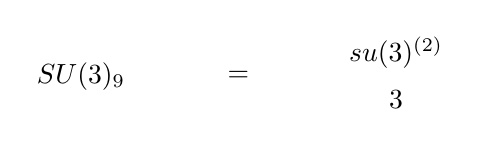
\begin{tikzpicture}
\draw (0, 0) node {$ SU(3)_9 $}
(2, 0) node {$ = $}
(4, 0.3) node {$ \mathfrak{su}(3)^{(2)} $}
(4, -0.3) node {$ 3 $};
\end{tikzpicture}
\end{align}
We follow the notations in \cite{Bhardwaj:2019fzv} to denote 6d theories. It is geometrically engineered by gluing $ \mathbb{F}_{10} $ and $ \mathbb{F}_0 $ \cite{Jefferson:2018irk}:
\begin{align}\label{eq:su3_9_geo}
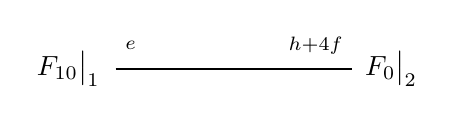
\begin{tikzpicture}
\draw[thick](-3,0)--(0,0);	
\node at(-3.6,0) {$\mathbb{F}_{10}{}\big|_1$};
\node at(-2.8,0.3) {${}_e$};
\node at(0.5,0) {$\mathbb{F}_{0}{}\big|_2$};
\node at(-0.45,0.3) {${}_{h+4f}$};
\end{tikzpicture} 
\end{align}
In geometry, the duality is simply the exchange of the base and the fiber classes in $\mathbb{F}_0$.
We will solve the blowup equations for this theory in both 5d and 6d frames and compare the results.

In the 5d $SU(3)_9$ theory, the effective prepotential $\mathcal{E}$ is given by
\begin{align}\label{eq:su3_9_prepotential}
\mathcal{E} &= \frac{1}{\epsilon_1 \epsilon_2} 
\left( \mathcal{F} - \frac{\epsilon_1^2  + \epsilon_2^2}{12}(\phi_1 + \phi_2) +\epsilon_+^2 (\phi_1 + \phi_2) \right), \\ 
6 \mathcal{F} &=  6m\big(\phi_1^2 - \phi_1 \phi_2 + \phi_2^2\big) +8\phi_1^3 + 24\phi_1^2 \phi_2 - 30\phi_1 \phi_2^2 + 8\phi_2^2  \ , \nonumber 
\end{align}
where $m$ is the gauge coupling. The GV-invariant of this theory takes the same form of \eqref{eq:SU3_k_GV}. It is convenient to use volumes of three independent 2-cycles in the geometry \eqref{eq:su3_9_geo} as the basis of states in the GV-invariant,
\begin{align}\label{eq:su3_9_vol}
\vol (f_1) =  2\phi_1 - \phi_2, \quad
\vol (f_2) = -\phi_1 + 2\phi_2, \quad
\vol (e_2) = -4\phi_1 + 2\phi_2 + m\ .
\end{align}
Unlike the other $SU(3)_\kappa$ theories with $|\kappa|\le 7$, this theory has only one set of consistent magnetic fluxes respecting the $ SU(3) $ structure:
\begin{align}\label{eq:MFforSU3_9}
	n_1,n_2\in \mathbb{Z} \ , \quad B_m = 0 \ .
\end{align}
This set of fluxes gives rise to a unity blowup equation. As we discussed already, a single unity blowup equation is enough to compute the BPS invariants. By solving the unity blowup equation, we find the BPS spectrum of the $SU(3)_9$ theory listed in Table~\ref{table:SU3_9}.
\begin{table}
	\centering
	\begin{tabular}{|c|C{28ex}||c|C{28ex}|} \hline
		$\mathbf{d}$ & $\oplus N_{j_l, j_r}^{\mathbf{d}} (j_l, j_r)$ & $\mathbf{d}$ & $\oplus N_{j_l, j_r}^{\mathbf{d}} (j_l, j_r)$ \\ \hline
		$(1, 0, 0)$ & $(0, \frac{1}{2})$ &$ (1, 0, 1)$ & $(0, \frac{3}{2})$ \\ \hline
		$(1, 0, 2)$ & $(0, \frac{5}{2})$ & $(1, 1, 0)$ & $(0, \frac{1}{2})$ \\ \hline
		$(1, 1, 1)$ & $(0, \frac{1}{2}) \oplus (0, \frac{3}{2})$ & $(1, 1, 2)$ & $(0, \frac{3}{2}) \oplus (0, \frac{5}{2})$ \\ \hline
		$(1, 2, 1)$ & $(0, \frac{1}{2}) \oplus (0, \frac{3}{2})$ & $(1, 2, 2)$ & $(0, \frac{1}{2}) \oplus (0, \frac{3}{2}) \oplus (0, \frac{5}{2})$ \\ \hline
		$(2, 0, 1)$ & $(0, \frac{5}{2})$ & $(2, 0, 2)$ & $(0, \frac{5}{2}) \oplus (0, \frac{7}{2}) \oplus (\frac{1}{2}, 4)$ \\ \hline
		$(2, 1, 1)$ & $(0, \frac{3}{2}) \oplus (0, \frac{5}{2})$ & $(2, 1, 2)$ & $(0, \frac{3}{2}) \oplus 3(0, \frac{5}{2}) \oplus 2(0, \frac{7}{2}) \oplus (\frac{1}{2}, 3) \oplus (\frac{1}{2}, 4)$ \\ \hline
		$(2, 2, 1)$ & $(0, \frac{1}{2}) \oplus (0, \frac{3}{2}) \oplus (0, \frac{5}{2})$ & $(2, 2, 2)$ & $(0, \frac{1}{2}) \oplus 3(0, \frac{3}{2}) \oplus 4(0, \frac{5}{2}) \oplus 2(0, \frac{7}{2}) \oplus (\frac{1}{2}, 2) \oplus (\frac{1}{2}, 3) \oplus (\frac{1}{2}, 4)$ \\ \hline
		$ (3, 0, 1) $ & $ (0, \frac{7}{2}) $ & $ (3, 0, 2) $ & $ (0,\frac{5}{2}) \oplus (0,\frac{7}{2}) \oplus 2(0,\frac{9}{2}) \oplus (\frac{1}{2},4) \oplus (\frac{1}{2},5) \oplus (1,\frac{11}{2}) $ \\ \hline
		$ (3, 1, 1) $ & $ (0,\frac{5}{2}) \oplus (0,\frac{7}{2}) $ & $ (3, 1, 2) $ & $ (0,\frac{3}{2}) \oplus 3(0,\frac{5}{2}) \oplus	5(0,\frac{7}{2}) \oplus 3(0,\frac{9}{2}) \oplus (\frac{1}{2},3) \oplus 3(\frac{1}{2},4) \oplus 2(\frac{1}{2},5) \oplus (1,\frac{9}{2}) \oplus (1,\frac{11}{2}) $ \\ \hline
		$ (3, 2, 1) $ & $ (0, \frac{3}{2}) \oplus (0, \frac{5}{2}) \oplus (0, \frac{7}{2}) $ & $ (3, 2, 2) $ & $ (0,\frac{1}{2}) \oplus 3(0,\frac{3}{2}) \oplus 8(0,\frac{5}{2}) \oplus 7(0,\frac{7}{2}) \oplus 4(0,\frac{9}{2}) \oplus (\frac{1}{2},2) \oplus 3(\frac{1}{2},3) \oplus 4(\frac{1}{2},4) \oplus 2(\frac{1}{2},5) \oplus (1,\frac{7}{2}) \oplus (1,\frac{9}{2}) \oplus (1,\frac{11}{2}) $ \\ \hline
	\end{tabular}
	\caption{BPS spectrum of $SU(3)_9$ theory for $d_1 \leq 3$ and $ d_2, d_3 \leq 2 $. Here, $\mathbf{d} = (d_1, d_2, d_3)$ labels BPS states with charge $d_1 e_2 + d_2 f_1 + d_3 f_2$ cycle.} \label{table:SU3_9}
\end{table}

We now perform a similar computation in the perspective of the 6d $SU(3)$ gauge theory with $\mathbb{Z}_2$ twist. In the 6d frame, the volumes of 2-cycles in the geometry are 
\begin{equation}
	{\rm vol}(f_1) = \frac{\tau}{4} - \phi_1 \ , \quad {\rm vol}(f_2) = 2\phi_1 \ , \quad {\rm vol}(e_2) = 3\phi_0+2\phi_1-\frac{\tau}{2}\ .
\end{equation}
The effective prepotential in this frame is given in \eqref{eq:E-SU3-Z2} with a shift $\phi_0 \rightarrow \phi_0-\frac{1}{16}\tau$. 

The GV-invariant for this 6d theory can be written as
\begin{align}
Z_{GV}(\Phi, \phi_1, \tau; \epsilon_{1,2})
= \mathcal{Z}_{\mathrm{pert}}(\phi_1, \tau; \epsilon_{1,2})  \qty(1 + \sum_{k=1}^{\infty} e^{-k \Phi} Z_k(\phi_1, \tau, \epsilon_{1,2}))\ ,
\end{align}
where $ Z_k(\phi_1, \tau, \epsilon_{1,2}) $ is the $ k $-string elliptic genus and $\Phi\equiv 3\phi_0-\tau/2$ which is the string number fugacity. Here, the perturbative part can be read off from the 6d $SU(3)$ vector multiplets under the $\mathbb{Z}_2$ automorphism twist, which is given by
\begin{align}
\mathcal{Z}_{\mathrm{pert}}
= \PE \qty[ -\frac{1+p_1 p_2}{(1-p_1)(1-p_2)} \frac{1}{1-q} \qty(e^{-2\phi_1} + (q^{1/4}+q^{3/4})(e^{-\phi_1}+e^{\phi_1}) + q e^{2\phi_1}) ] , 
\end{align}
where $ q = e^{-\tau} $. See Appendix~\ref{appendix:1-loop} for more details.

There are three sets of consistent magnetic fluxes preserving the affine $A^{(2)}_2$ algebra structure:
\begin{align}
	n_1 \in \mathbb{Z}\ , \quad B_\tau = 0  \ , \quad n_0 \in \mathbb{Z}+B_0 \ \ {\rm with } \ \  B_0=0,1/3,2/3 \ .
\end{align}
Then the elliptic genus can be found by solving three unity blowup equations from these three flux sets. For example, the blowup equations at 1-string order are
\begin{align}
&\Lambda(\tau; \epsilon_1, \epsilon_2) \hat{Z}_1(\phi_1, \tau; \epsilon_1, \epsilon_2) \nonumber \\
&= \sum_{\vec{n} = (n, 2n)} e^{-V} \frac{\hat{\mathcal{Z}}_{\mathrm{pert}}^{(N)} \hat{\mathcal{Z}}_{\mathrm{pert}}^{(S)}}{\hat{\mathcal{Z}}_{\mathrm{pert}}} \qty(p_1^{3n + B_0} \hat{Z}_1(\phi_1, \epsilon_1, \epsilon_2 - \epsilon_1) + p_2^{3n + B_0} \hat{Z}_1(\phi_1, \epsilon_1 - \epsilon_2, \epsilon_2) ) \nonumber \\
& \qquad + \sum_{\vec{n} = (n, 2n \pm 1)} e^\Phi e^{-V} \frac{\hat{\mathcal{Z}}_{\mathrm{pert}}^{(N)} \hat{\mathcal{Z}}_{\mathrm{pert}}^{(S)}}{\hat{\mathcal{Z}}_{\mathrm{pert}}} \ .
\end{align}
Here the prefactor can be computed by collecting all $\phi_i$ independent terms in the blowup equation as follows:
\begin{align}
\Lambda(\tau; \epsilon_1, \epsilon_2) = \sum_{\vec{n} = (n, 2n)} e^{-V} \ .
\end{align}
The solution at 1-instanton string is then given by
\begin{align}
Z_1(\phi_1, \tau; \epsilon_1, \epsilon_2)
&= \frac{e^{-2\phi_1} p_1 p_2 (1+p_1 p_2)}{(1-p_1)(1-p_2) (e^{-2\phi_1} - p_1 p_2) (1-e^{-2\phi_1} p_1 p_2)} \nonumber \\
& \quad + \frac{e^{-\phi_1}(1+e^{-2\phi_1}) p_1 p_2 (1+p_1 p_2)}{(1-p_1) (1-p_2) (e^{-2\phi_1} - p_1 p_2) (1-e^{-2\phi_1} p_1 p_2)} q^{1/4} \nonumber \\
& \quad + \frac{e^{-2\phi_1} (1 + 2p_1 p_2 + 2p_1^2 p_2^2 + p_1^3 p_2^3)}{(1-p_1)(1-p_2) (e^{-2\phi_1} - p_1p_2)(1-e^{-2\phi_1} p_1 p_2)} q^{1/2} + \cdots \ .
\end{align}
This is in perfect agreement with the BPS spectrum of the $ SU(3)_9 $ theory given in Table \ref{table:SU3_9} and also topological vertex as well as the ADHM calculations \cite{Kim:2021cua}.